\section{Supplementary methods}

These sections provide more detailed descriptions of the mathematical models and numerical approximations considered.

\subsection{Mixed-dimensional transport and flow equations}
\label{sec:app:more_maths}

\subsubsection{Notation}

In terms of geometrical domains, we consider the parenchyma
$\Omega_{\rm PAR} \subset \R^3$ and CSF spaces $\Omega_{\rm CSF}
\subset \R^3$ with $\Omega = \Omega_{\rm PAR} \cup \Omega_{\rm CSF}$
(\Cref{fig:results1}A, \Cref{fig:csf}A--C). The coordinates in these
3D domains is denoted by $x$. The interface between the parenchyma and
CSF spaces is given by $\partial \Omega_{\rm PAR} \cap \partial
\Omega_{\rm CSF}$ and we separate it as two parts: the surface of the
lateral ventricles $\Gamma_{\rm LV}$ and the remaining pial interface
$\Gamma_{\rm pia}$ (thus $\partial \Omega_{\rm CSF} \bigcap \partial
\Omega_{\rm PAR} = \Gamma_{\rm LV} \cup \Gamma_{\rm pia}$). The
remaining, outer, boundary of $\Omega_{\rm CSF}$ is again separated
into two parts: $\Gamma_{\rm SSAS}$ represents the lower interface
towards the spinal subarachnoid space (SSAS), while $\Gamma_{\rm AM}$
is the outer interface towards the arachnoid and dura
membranes. $\Gamma_{\rm AM}$ is further subdivided into its lower and
upper parts: $\Gamma_{\rm AM-L}$ and $\Gamma_{\rm AM-U}$. The boundary
towards the spinal cord is denoted by $\Gamma_{\rm{SC}}$ and given by
$\Gamma_{\rm{SC}} = \partial \Omega_{\rm PAR} \setminus \partial
\Omega_{\rm CSF}$.

In addition, we consider two sets of perivascular networks: a
periarterial network $\Lambda_a$ represented by the (connected)
centerlines $\Lambda^i_{a}$ of the arterial tree, and a perivenous
network $\Lambda_v$ associated with the centerlines $\Lambda^i_{v}$
of the veins. Recall that we represent the vascular domains as the
union of cylindrical vessels of radius $R_1^i$ surrounding the
centerlines $\Lambda^i$. Moreover, we consider the surrounding
perivascular spaces as the union of annular cylinders $\Omega^i$ of
inner radius $R_1^i$ and outer radius $R_2^i > R_1^i$ and thus of
width $R_2^i - R_1^i$, and remark that we interpret $R^i_2$ and $R^i_1$ as temporal averages (fixed in time), as the pulsations considered in \Cref{sec:app:peristalsis} are beyond the temporal resolution of our model. We denote the outer lateral surface of the
periarterial and perivenous spaces by $\Gamma_a$ and $\Gamma_v$,
respectively. We omit the subscript $a$ or $v$ when referring to any
such network, vessel segment or perivascular outer surface. We assume
that $\Lambda$ is parametrized by the coordinate $s$, and with a minor
abuse of notation, simply write $s \in \Lambda$ to represent the point
${\bm \lambda}(s)$ on $\Lambda$ corresponding to $s$. Finally, we view
each perivascular network both as a geometric domain and as a directed
graph with the centerlines $\{ \Lambda^i \}$ as oriented edges and the
connections as nodes $\mathcal{V}$.

\subsubsection{Solute transport and exchange in intracranial domains (3D) and perivascular networks (1D)}
\label{sec:app:transport_eqs}

In this section, we describe the mathematical
model~\eqref{eq:multi_transport}, the associated definitions,
interface and boundary conditions in further detail. We refer to the
main text for explicit parameter values while giving the general,
abstract form here, and to the reference~\cite{masri2024modelling, laurino2019derivation} for
the derivation and analysis of this 3D-1D model. Recall that we model
a concentration field $c = c(x, t)$ for $x \in \Omega$ and $t > 0$
defined in $\Omega_{\rm PAR}$ and $\Omega_{\rm CSF}$ separately. In
each of these domains, $c$ satisfies
%\mer{MER: Rami asks if it should be a $\phi$ in the advective term here. We can include it, or drop it, but in the latter case, perhaps we should clarify that u is an average/superficial/Darcy velocity.}
\begin{equation}
  \partial_t (\phi c) - \nabla \cdot (D \nabla (\phi c) ) + \nabla \cdot (\bm u c ) + \xi (\overline{c} - \hat c ) \delta_\Gamma
  %= f
   = 0
  \quad \quad \mathrm{in} \quad \Omega_{\rm CSF}, \Omega_{\rm{PAR}}.
  \label{eq:3d_pde}
\end{equation}
In~\eqref{eq:3d_pde}, $\phi$ is the fluid volume fraction (also known as the porosity) defined in the parenchyma ($\phi \ll 1$ in $\Omega_{\rm PAR}$) and in the CSF spaces ($\phi = 1$ in $\Omega_{\rm CSF}$). In the parenchyma, $\phi$ represents the extracellular space volume fraction, and thus $c$ here generally represents the intrinsic (in contrast to the superficial) concentration~\cite{sykova2008diffusion}. Moreover, $D$ is the effective diffusion coefficient of the relevant solute in the respective media which takes different values over the CSF spaces and the parenchyma, depending on tortuosity~\cite{sykova2008diffusion} and dispersive effects; and $\bm u$ is a convective velocity field representing the flow of CSF in $\Omega_{\rm CSF}$ and the flow of ISF in $\Omega_{\rm PAR}$. $\xi$ models a transfer or exchange parameter between the 3D domain ($\Omega_{\rm PAR}$ or $\Omega_{\rm CSF}$) and the perivascular networks $\Lambda_a, \Lambda_v$. To summarize,
\begin{equation*}
\phi =  \begin{cases}
  1  & \mathrm{in} \;  \Omega_{\rm{CSF}} \\ 
  \phi_{\rm{PAR}} & \mathrm{in} \; \Omega_{\rm{PAR}} 
  \end{cases}, \; 
D = \begin{cases}
  D_{\rm{CSF}} & \mathrm{in} \;  \Omega_{\rm{CSF}} \\ 
  D_{\rm{PAR}} & \mathrm{in} \; \Omega_{\rm{PAR}} \end{cases}, \; 
  \quad \bm u  = \begin{cases}
  \bm{u}_{\rm{CSF}} & \mathrm{in} \; \Omega_{\rm{CSF}} \\ 
  \bm{u}_{\rm{PAR}} & \mathrm{in} \; \Omega_{\rm{PAR}} 
\end{cases}, \; 
\xi = \begin{cases}
  \xi_{\rm{CSF}} & \mathrm{if} |\Omega^i \cap \Omega_{\rm{CSF}}| \neq 0 \\
  \xi_{\rm{EF}} & \mathrm{if} |\Omega^i \cap \Omega_{\rm{PAR}}| \neq 0  
\end{cases} . 
\end{equation*}
In the above, $\xi$ is defined segment-wise: for each centerline $\Lambda^i$ with surrounding PVS $\Omega^i$, $|\Omega^i \cap \Omega_{\rm{PAR}}|$ (resp. $|\Omega^i \cap \Omega_{\rm{CSF}}|$) is nonzero whenever $\Omega^i$ intersects $\Omega_{\rm{PAR}}$ (resp. $\Omega_{\rm{CSF}}$). If the surrounding PVS intersects both, then we set $\xi = \xi_{\rm EF}$ if $\Omega^i$ mainly ($80$ percent) intersects $\Omega_{\rm{PAR}}$, in which case the interaction with $\Omega_{\rm{CSF}}$ is ignored; otherwise, we set $\xi = \xi_{\rm CSF}$. 
 
Also in~\eqref{eq:3d_pde}, the notation $\overline{c}$ denotes a lateral average of the concentration over the outer perivascular surfaces, defined for each centerline $\Lambda^i$ and each point $s \in \Lambda^i$ by
\begin{equation*}
  \overline{c}(s) = \frac{1}{P(s)} \int_{\partial \Theta_2^i(s)} c 
\end{equation*}
where $\partial \Theta_2^i(s)$ is the outer boundary of the cross-section $\Theta(s)$ of the PVS $\Omega^i$ at $s$ and $P(s)$ is the perimeter of $\Theta(s)$. Moreover, for both the periarterial and perivenous networks ($\Lambda_a, \Lambda_v$ with outer PVS boundaries $\Gamma_a, \Gamma_v$), the term $\delta_\Gamma$ is concentrated on the outer lateral surfaces of the PVSs, and defined in terms of its action on any sufficiently smooth function $v : \Omega \rightarrow \R$
%and for each $\Lambda^i \subseteq \Lambda$ with PVS $\Omega^i$ and outer lateral surface $\Gamma^i = \partial \Omega^i_2$
such that
\begin{equation*}
  \langle \xi (\overline{c} - \hat c ) \delta_\Gamma, v \rangle =
  \int_{\Lambda} P \xi (\overline{c} - \hat c ) \overline{v}, 
\end{equation*}
under the assumption that $\xi$ is constant on each $\partial
\Theta_2^i$.
%% , since:
%% \begin{multline}
%%   \int_{\Omega} \xi (\overline{c} - \hat c ) \delta_\Gamma (v) =
%%   \int_{\Gamma} \xi (\overline{c} - \hat c ) \delta_\Gamma (v) =
%%   \sum_i \int_{\Gamma^i} \xi (\overline{c} - \hat c ) \delta_\Gamma (v) = 
%%   \sum_i \int_{\Lambda^i} \int_{\partial \Theta_2^i} \xi (\overline{c} - \hat c ) \delta_\Gamma (v) = \\
%%   \sum_i \int_{\Lambda^i} \left (  \xi (\overline{c} - \hat c ) \int_{\partial \Theta_2^i} \delta_\Gamma (v) \right ) =
%%   \sum_i \int_{\Lambda^i} P \xi (\overline{c} - \hat c ) \overline{v} =
%%   \int_{\Lambda} P \xi (\overline{c} - \hat c ) \overline{v} .
%% \end{multline}
%% \mer{MER: The previous was:
%% \begin{equation}
%%   \xi (\overline{c} - \hat c ) \delta_\Gamma (v) = \int_{\Lambda} P \xi ( \overline{c} - \hat c ) \overline{v} .
%% \end{equation}
%% }

On the interface between the brain and the CSF spaces
$\Gamma_{\mathrm{pia}} \cup \Gamma_{\rm LV}$, we prescribe the
following interface conditions, which represent a semi--permeable
interface, writing $c|_{\Omega_{\rm PAR}} = c_{\rm PAR}$ and
$c|_{\Omega_{\rm CSF}} = c_{\rm CSF}$:
%% \begin{subequations}
%% \begin{alignat}{2}
%% (-D \nabla (\phi c_{\rm{PAR}}) + \bm u_{\rm{PAR}} c_{\rm{PAR} }) \cdot \bm{n} &= - (- D (\phi \nabla c_{\rm{CSF}}) + \bm u_{\rm{CSF}} c_{\rm{CSF}} ) \cdot \bm{n} &&  \quad  \mathrm{on} \quad \Gamma_{\rm pia} \cup \Gamma_{\mathrm{LV}} ,  \\  
%% (-D \nabla ( c_{\rm{PAR}}) + \bm u_{\rm{PAR}} c_{\rm{PAR} }) \cdot \bm{n} & = \beta_{\rm{pia}} (c_{\rm PAR} - c_{\mathrm{CSF}}) &&  \quad  \mathrm{on} \quad \Gamma_{\rm pia} \cup \Gamma_{\mathrm{LV}} ,  
%% \end{alignat} 
%% \end{subequations}
\begin{subequations}
  \begin{alignat}{2}
  (-D \nabla (\phi c) + \bm u c)|_{\Omega_{\rm PAR}} \cdot \bm{n}
  &= - (-D \nabla (\phi c) + \bm u c)|_{\Omega_{\rm CSF}} \cdot \bm{n}
  &&  \quad  \mathrm{on} \quad \Gamma_{\rm pia} \cup \Gamma_{\mathrm{LV}} ,  \\  
  (- D \nabla (\phi  c) + \bm u c)|_{\Omega_{\rm PAR}} \cdot \bm{n} & = \beta_{\rm{pia}} (c_{\rm PAR} - c_{\mathrm{CSF}}) &&  \quad  \mathrm{on} \quad \Gamma_{\rm pia} \cup \Gamma_{\mathrm{LV}} ,  
\end{alignat} 
  \label{eq:3d_interface}%
\end{subequations}%
where $\bm{n} = \bm{n}_{\rm PAR}$ is the normal vector field defined
over the interface, outward-pointing when viewed from $\Omega_{\rm
  PAR}$, and $\beta_{\mathrm{pia}} \geqslant 0$ is a permeability
constant.

We supplement~\eqref{eq:3d_pde} and~\eqref{eq:3d_interface} with the following boundary conditions representing a given molecular influx at $\Gamma_{\rm SSAS}$, molecular efflux at a constant update rate $\beta_{\rm exit}$ at $\Gamma_{\rm AM-U}$, and no influx or efflux elsewhere from the CSF spaces.
\begin{subequations}
\begin{alignat}{2}
(D \nabla (\phi c) - \bm u c ) \cdot \bm{n} &= g_{\mathrm{influx}} &&  \quad  \mathrm{on} \quad \Gamma_{\rm SSAS},  \\ 
% (-D \nabla (\phi c) + \bm u c ) \cdot \bm{n}_{\Gamma_{\rm SAS}} &= 0 &&  \quad  \mathrm{on} \quad \Gamma_{\rm SAS}^{\mathrm{out}}  \\ 
(-D \nabla (\phi c) + \bm u c ) \cdot \bm{n} & = \beta_{\rm exit} c  &&  \quad  \mathrm{on} \quad \Gamma_{\rm AM-U},  \\ 
(-D \nabla (\phi c) + \bm u c ) \cdot \bm{n} & = 0  &&  \quad  \mathrm{on} \quad \Gamma_{\rm AM-L} \cup \Gamma_{\rm SC}  .
\end{alignat} 
\label{eq:3d_bcs}
\end{subequations}
where again $\bm n$ denotes the outward-pointing boundary normal.

The concentration $\hat{c} = \hat{c}(s, t)$ in the periarterial and
perivenous networks ($s \in \Lambda_a, s \in \Lambda_v$), entering
in~\eqref{eq:3d_pde}, represents the concentration in the perivascular
space averaged over each perivascular cross-section and is governed by 
\begin{equation}
  \partial_t (A  \hat c) - \partial_s( \hat D A \partial_s \hat c  ) + \partial_s(A \hat u \hat c )  +  \xi P (\hat c - \overline{c}) = 0
  \qquad \text{in} \quad \Lambda_a, \Lambda_v ,
\label{eq:1d_pde}
\end{equation}
where in $\Lambda_a, \Lambda_v$ refers to in each $\Lambda^i$ in each
of these networks. In~\eqref{eq:1d_pde}, $A = A(s)$ is defined as the
PVS cross-sectional area; i.e.,~for each $s \in \Lambda^i$ with
associated PVS $\Omega^i$, the area of the cross-section
$\Theta^i(s)$. Also, $\hat{D}$ is the effective diffusion coefficient,
and $\hat{u}$ is a convective velocity representing an (average) CSF
flow velocity in the axial direction of the perivascular spaces.

To complete~\eqref{eq:1d_pde}, we prescribe bifurcation conditions at
internal nodes of the perivascular networks $\Lambda_a, \Lambda_v$ and
boundary conditions at the end nodes. To this end, define the set of
internal nodes $\mathcal{B} \subset \mathcal{V}$ as the set of nodes
that are connected to two or more edges and the set of end nodes as
$\mathcal{N} \subset \mathcal{V}$, write $\hat{c}^i =
\hat{c}|_{\Lambda^i}$, and for $y\in\mathcal{B}$ let $\mathcal{E}(y)$ denote the set of
(two or three) edges in $\{\Lambda^i\}$ sharing the node $y$. To
impose continuity of the concentrations, we set that the
concentrations when viewed from each edge must match at nodes:
\begin{equation}
  \hat{c}^i (y) = \hat{c}^j(y)
  \qquad \foralls \Lambda^i, \Lambda^j \in \mathcal{E}(y)
  \qquad \foralls y \in \mathcal{B} .
  \label{eq:conc_continuity}
\end{equation}
Moreover, to ensure mass conservation, we set that the flux
going in and out at nodes should add to zero, or more precisely, that
for each $y \in \mathcal{B}$:
\begin{equation}
  \sum_{\Lambda^i \in \mathcal{E}(y)}
  \left (\hat{D}^i A^i \partial_s \hat{c}^i (y) - A^i \hat u^i(y) \hat{c}^i(y) \right ) n^i(y)
  = 0.
  \label{eq:flux_conservation}
\end{equation}
Here the (normal ``vector") function $n^i$ takes the values in $\left\{-1, 1\right\}$ and 
defines an orientation of vertices of edge $\Lambda^i$. Specifically, for an edge $\Lambda^i$ oriented from $y_{\rm in}$ to $y_{\rm out}$ we set 
\begin{equation}
  n^i(y_{\rm in}) = 1,\quad
  n^i(y_{\rm{out}}) = -1. %\quad
  %\mk{n^i(y) = 0 \quad \foralls y \in 
  %\mathcal{V} \backslash \{ y_{\rm in}, y_{\rm out} \} }.  
\label{eq:def:sign}
\end{equation}
%\mk{Why do we need the normal on non-IO vertices?}

Finally, we impose a homogeneous Neumann condition at all network end
nodes to augment~\eqref{eq:1d_pde}:
\begin{equation}
    \hat D A \partial_s (\phi \hat c) - A \hat u \hat c  = 0 \quad \mathrm{on} \quad \mathcal{N}.
    \label{eq:1d_bcs}
\end{equation}
This no-flux condition states that the network end nodes represent
barriers for molecular efflux into or out of the perivascular network,
and thus that all solute exchange between the PVSs and their
surroundings takes place via the lateral outer PVS surface and is
regulated by the exchange parameter $\xi$ cf.~\eqref{eq:3d_pde}
and~\eqref{eq:1d_pde}. Larger particles have been observed to
accumulate within the PVS as the surface arteries penetrate into the
brain parenchyma~\cite{mestre2018flow, bedussi2018paravascular},
and~\eqref{eq:1d_bcs} is appropriate to represent such
behavior. However, to represent a continuously extending PVSs also
along penetrating vessels, this condition should be revisited.

\subsubsection{Modelling CSF flow via the incompressible Stokes equations}
\label{sec:app:csf_flow}
The time-independent, incompressible Stokes equations model the flow
of an incompressible Newtonian fluid at low Reynolds numbers, and read
as follows: over the domain $\Omega_{\rm CSF} \subset \R^3$, find the
velocity vector field $\bm u : \Omega_{\rm CSF} \rightarrow \R^3$ and
the pressure field $p : \Omega_{\rm CSF} \rightarrow \R$ such that
\begin{subequations}
  \begin{alignat}{2}
    - \mu \Delta \bm u  + \nabla p &=  0 \quad && \text{ in } \Omega_{\rm CSF},
    \label{eq:momentum_equation} \\ 
    \nabla \cdot \bm u &= 0 \quad && \text{ in } \Omega_{\rm CSF}
    \label{eq:divergence_equation} .
  \end{alignat}
  \label{eq:stokes}%
\end{subequations}%
In addition, we impose the following boundary conditions to model flow
induced by CSF production in the choroid plexus with $\Gamma_{\rm AM-U}$ as the main efflux site:
\begin{subequations}
  \begin{alignat}{2}
( \mu \nabla \bm u \cdot \bm{n} - p \bm n) \cdot \bm n  &= -R_0 ( \bm u \cdot \bm n ), \quad \bm u \cdot \bm t = 0
    && \text{ on } \Gamma_{\mathrm{AM-U}}, \\
    \bm u &= 0 && \text{ on } \Gamma_{\mathrm{AM-L}}\cup\Gamma_{\rm{pia}}\cup\Gamma_{\rm{SSAS}}, \\
    %\bm u &= 0 && \text{ on } \Gamma_{\rm{pia}}, \\
    %\bm u &= 0 && \text{ on } \Gamma_{\rm{SSAS}}, \\
    \bm u \cdot \bm n & = \frac{1}{ |\Gamma_{\rm LV}|}  u_{\rm in}, \quad \bm u \cdot \bm t = 0 \quad && \text{ on } \Gamma_{\rm{LV}} ,  
  \end{alignat}
  \label{eq:stokes_bcs}%
\end{subequations}%
where $\bm n$ and $\bm t$ denote the unit outward normal and tangent vectors to the boundary respectively,  $\mu$ is the (dynamic) CSF viscosity, $R_0 > 0$ is a resistance parameter for CSF efflux, and $u_{\rm in}$ is a given fluid influx, here across the lateral ventricle wall $\Gamma_{\rm LV}$. We consider alternative variations of these boundary conditions in connection with estimating dispersion effects induced by CSF pulsatility, see~\Cref{sec:app:dispersion}.

%% We consider non-zero convection in the CSF space $u_{\rm CSF} \not = 0$ in \eqref{eq:multi_transport_3d} resulting from steady state CSF production.  Recall that $\Omega_{\mathrm{CSF}}$ represents the CSF space and that $\Gamma_{\mathrm{skull^{u/l}}}$ and $\Gamma_{\mathrm{pia}}$, $\Gamma_{\mathrm{LV}}$ represent the boundaries facing the upper and lower parts of the dura, the pia and the lateral ventricles, respectively.  Assuming CSF production in the choroid plexus located at the lateral ventricle wall, we solve the  steady state Stokes equations for the velocity and the pressure $(\bm u_{\mathrm{CSF}}, p_{\mathrm{CSF}})$ in the CSF domain: 

\subsubsection{Steady flow in perivascular networks induced by pressure differences}
\label{sec:app:hydraulic_network}

To model steady flow induced by pressure differences between end nodes
in a perivascular network $\Lambda$, with edges $\{\Lambda^i\}_i$,
internal nodes $\mathcal{B}$ and end nodes $\mathcal{N}$, we consider
the following system of hydraulic network
equations~\cite{tithof2022network, daversin2022geometrically,
  gjerde2024directional}. The unknowns are the PVS flux $\hat{q} :
\Lambda \rightarrow \R$ and pressure $\hat{p} : \Lambda
\rightarrow \R$, which represent the fluid flux and the average
pressure across cross-sections of the PVSs, respectively. These are
defined for each $\Lambda^i$ by solving:
\begin{subequations}
\begin{alignat}{2}
  \hat{q} + \frac{A \kappa}{\mu} \partial_{s} \hat{p} & = 0 &&
  \quad \text{ in } \Lambda^i , \\ 
  - \partial_s \hat{q} & = 0 &&
  \quad \text{ in } \Lambda^i ,  
\end{alignat} 
\label{eq:1d_flow}%
\end{subequations}%
where $A$ is the area of the PVS cross-sections, $\mu$ is the CSF viscosity as before, and $\kappa$ is derived from an assumption of Poiseuille flow in the annular cross-section of the PVS as~\cite{tithof2022network}: 
\begin{equation}
\kappa = \frac18 \left( R_2^2 + R_1^2 - \frac{1}{\ln(R_2/R_1)} (R_2^2- R_1^2) \right). 
\end{equation}
The PVS flux $\hat{q}$ and the associated average PVS velocity in the
axial direction $\hat{u}$ are directly related by the cross-sectional area
\begin{equation}
  \hat{q}^i = A^i \hat{u}^i \qquad \foralls \Lambda^i.
\end{equation}

In addition, to complete~\eqref{eq:1d_flow}, we impose continuity of
the fluid pressure and conservation of flux at each internal node. Write
$\hat{p}^i = \hat{p}|_{\Lambda^i}$. These conditions then read as: for
each $y \in \mathcal{B}$ with connected edges $\mathcal{E}(y)$:
\begin{subequations}
\begin{align}
  \hat{p}^i(y) &= \hat{p}^j(y) \qquad \foralls \Lambda^i, \Lambda^j \in \mathcal{E}(y), \\
  \sum_{\Lambda^i \in \mathcal{E}(y)} \hat{q}^i n^i(y) &= 0  .
\end{align}
\label{eq:1d_flow:bifurcations}
\end{subequations}
where $n^i$ is as defined by~\eqref{eq:def:sign}. Finally, to drive this flow, we impose given fluid pressures $p_0$ at the
network end nodes:
\begin{equation}
  \hat{p}(y) = p_0(y) \qquad y \in \mathcal{N} .
  \label{eq:1d_flow:bcs}
\end{equation}
In the case where modelling flow in the perivascular networks
$\Lambda_a, \Lambda_v$ induced by CSF production, we impose the fluid
pressure $p_{\rm CSF}$ computed in the CSF spaces $\Omega_{\rm CSF}$
(and its harmonic extensions into $\Omega_{\rm PAR}$) as the given
fluid pressures $p_0$. Note that we here consider steady PVS flow in a
non-moving domain; the effect of domain motion is addressed
in~\Cref{sec:app:peristalsis}.

\subsection{Numerical solution of the transport and flow equations}
\label{sec:app:details_numerical_method}

We solve the models presented in~\Cref{sec:app:more_maths} numerically
using finite element methods. The following subsections provide more
details, model-by-model.

\subsubsection{Computational mesh entities: definitions and common notation}

We consider a mesh $\mathcal{T} = \{ E \}$ of $\Omega = \Omega_{\rm
  PAR} \cup \Omega_{\rm CSF}$, consisting of tetrahedral mesh cells
$E$, and conforming to the domains $\Omega_{\rm PAR}$ and $\Omega_{\rm
  CSF}$ and to the CSF-brain interface $\Gamma_{\rm pia} \cup
\Gamma_{\rm LV}$. We denote the restriction of $\mathcal{T}$ to
$\Omega_{\rm PAR}$ and $\Omega_{\rm CSF}$ by $\mathcal{T}_{\rm PAR}$
and $\mathcal{T}_{\rm CSF}$, respectively. The collection of all
interior facets (i.e.~triangular faces of the tetrahedral mesh cells)
in $\mathcal{T}_{\rm PAR}$ and $\mathcal{T}_{\rm CSF}$ are denoted by
$\mathcal{F}_{i, \rm PAR}$ and $\mathcal{F}_{i, \rm CSF}$,
respectively. We define the union of facets interior both to
$\mathcal{T}_{ \rm PAR}$ and $\mathcal{T}_{ \rm CSF}$ as
$\mathcal{F}_i = \mathcal{F}_{i, \rm PAR} \cup \mathcal{F}_{i, \rm
  CSF}$. 

%Note in particular that $\mathcal{F}_i \cap \mathcal{F}_{pia}} =
%  \emptyset$.

%The restriction of $\mathcal{T}_h $ to $\Omega_{\mathrm{CSF}}$ is
%denoted by $\mathcal{E}_{h}$.

\subsubsection{Finite element solution of coupled 3D-1D solute transport equations }

We consider the system of coupled 3D-1D solute transport equations
given by~\eqref{eq:3d_pde} and~\eqref{eq:1d_pde} with the interface
conditions~\eqref{eq:3d_interface}, the bifurcation
conditions~\eqref{eq:conc_continuity}
and~\eqref{eq:flux_conservation}, and the boundary
conditions~\eqref{eq:3d_bcs} and~\eqref{eq:1d_bcs}. We discretize
these equations using an implicit finite difference scheme in time, 
a discontinuous Galerkin (DG) finite element method with upwinding in space for the 3D domain to accurately capture sharp boundary layers, and a continuous Galerkin method for the 1D networks. We remark that the transport in the CSF spaces is highly convection dominated, with an average Péclet number of 402 and maximum of 9542 (assuming a characteristic length of $10\,$cm, and accounting for the increased diffusivity due to dispersion).

We first consider the discretization of~\eqref{eq:3d_pde} and
introduce the discrete space
\begin{equation}
  %V_h^k = \{c_h \in L^2(\Omega): \;  v_h \vert_E \in \mathbb{P}^k(E), \; E \in \mathcal{T}_h\}.
  V_h = \{c \in L^2(\Omega): \;  c \vert_E \in \mathrm{P}^1(E), \; E \in \mathcal{T}\} ,
\end{equation}
where $L^2(\Omega)$ is the space of square-integrable functions
defined over $\Omega$ and $\mathrm{P}^1(E)$ denotes the space of
polynomials of total degree $\leqslant 1$ defined over the tetrahedra
$E$. To discretize the diffusion term in~\eqref{eq:3d_pde}, we use a
symmetric weighted interior penalty DG formulation, referring
to~\cite{ern2009discontinuous} and \cite[Section
  4.5.2.3]{di2011mathematical} for details on this
method. Recall that $\phi$ is constant in each domain
  $\Omega_{\rm PAR}$ and $\Omega_{\rm CSF}$, and thus in particular
  that $\nabla (\phi c) = \phi \nabla c$ on each $E \in \mathcal{T}$.
Define for $c, v \in V_h^k$:
\begin{equation}
  a_h (c, v)
  =
  \sum_{E \in \mathcal{T}} \int_{E} D\phi \nabla c \cdot \nabla v
  - \sum_{F \in \mathcal{F}_i} \int_{F} \left( \{D \phi \nabla c \}_w \cdot \bm n_F [v]
  + \{D \phi \nabla v \}_w \cdot \bm n_F [c] \right) 
   + \sum_{F \in \mathcal{F}_i} \eta \frac{\gamma_{D,F}}{h_F} \int_{F} [c][v] 
  .
  \label{eq:dg_sip}
\end{equation}
In~\eqref{eq:dg_sip}, for each facet $F \in \mathcal{F}^i$ shared
between cells $E^1$ and $E^2$, we associate a  facet normal vector $\bm n_F$
pointing from $E^1$ to $E^2$. The facet diameter is denoted by $h_F$,
the jump $[\cdot]$ is given by $[v] = v|_{E^1} - v|_{E^2}$, and the
unweighted average $\{ \cdot \}$ and weighed average $\{ \cdot \}_w$
are defined as:
\begin{equation}
  \{v\} = \frac12 v |_{E^1} + \frac12 v |_{E^2}, \qquad
  \{v\}_{w} = \frac{\kappa_2}{\kappa_1 + \kappa_2} v |_{E^1} + \frac{\kappa_1}{\kappa_1 + \kappa_2} v |_{E^2}
  \quad \text{where} \quad \kappa_i = (D \phi) |_{E^i}.  
\end{equation}
The parameter $\gamma_{D,F}$ is the harmonic mean of the
porosity-weighted diffusion coefficient given by
\begin{equation}
  \gamma_{D,F} = \frac{2\kappa_1\kappa_2}{\kappa_1 + \kappa_2},
\end{equation}
and $\eta$ is a user-specified penalty parameter (we set $\eta=1000$). To discretize the convection term in~\eqref{eq:3d_pde}, we use
upwinding, see \cite[Section 2.3.1]{di2011mathematical} and the
references therein. For $c, v \in V_h^k$, define
\begin{equation}
  a_h^{\mathrm{up}}(c, v)
  = - \sum_{E \in \mathcal{T}} \int_E c\bm{u} \cdot \nabla v
  + \sum_{F \in \mathcal{F}_i } \int_F \{ \bm u  c\} \cdot \bm{n}_F [v] +
  \sum_{F \in \mathcal{F}_i} \int_F \frac{|\bm u \cdot \bm n_F|}{2} [c] [v] .
\end{equation}
Our discrete formulation for \eqref{eq:3d_pde} with the interface conditions~\eqref{eq:3d_interface} and boundary conditions~\eqref{eq:3d_bcs} and given initial conditions $c_h^0$ then reads: for $n = 1, 2, \dots$, with $t^n - t^{n-1} = \tau$, find $c_h^n \in V_h$ such that for all $v \in V_h$:
\begin{equation} \label{eq:3d_dg_disc}
  \int_{\Omega} \frac{1}{\tau} (\phi c_h^n - \phi c_h^{n-1}) v
  + a_h(c_h^n, v) + a_h^{\mathrm{up}}(c_h^n,v)
  + \int_{\Gamma_{\rm pia} \cup \Gamma_{\rm LV}} \beta_{\rm pia}[c_h^n][v] 
  + \int_{\Gamma_{\rm AM-U}} \beta_{\rm exit} c_h^n v 
  + \int_{\Lambda} \xi  P \left (\overline{c_h^n} - \hat c_h^n \right) \overline{v} 
  = 
  %\int_{\Omega} f^n v +
  \int_{\Gamma_{\rm SSAS}} g_{\rm influx} v
  %, \quad \forall v \in V_h^k
  .
\end{equation}

To discretize~\eqref{eq:1d_pde} with the bifurcation
conditions~\eqref{eq:conc_continuity}
and~\eqref{eq:flux_conservation}, and the boundary
conditions~\eqref{eq:1d_bcs}, we use the space of continuous piecewise
linear polynomials defined over $\Lambda$:
\begin{equation}
  \hat V_h
  = \{ v \in C^0(\Lambda), \; v \vert_{\Lambda^i} \in \mathrm{P}^1(\Lambda^i) \}, 
\end{equation}
where $\mathrm{P}^1(\Lambda^i)$ is the space of linear polynomials on each $\Lambda^i$. The discrete formulation then reads: for $n = 1,2,\ldots, $ find $\hat c_h^n \in \hat V_h$ such that for all $\hat v \in \hat V_h^k$: 
\begin{align}\label{eq:1d_dg_disc}
\int_{\Lambda}  \frac{1}{\tau}(A  \hat c_h^n - A \hat c_h^{n-1}) \hat v  + \int_{\Lambda} \hat D A \partial_s \hat c_h^n  \partial_s \hat v^n - \int_{\Lambda} A \hat u \hat c_h^n \partial_s \hat v   +  \int_{\Lambda} \xi P (\hat c_h^n - \overline{c_h^n}) \hat v +a_h^{\mathrm{stab}}(\hat u; \hat c, \hat v) = 0.  
\end{align}
 In the above, if $\hat u$ is non--zero on $\Lambda^i$, then the artificial diffusion $a_h^{\mathrm{stab}}$ stabilization term is nonzero  and is given below, for more details see for  \cite[Section 12.6]{quarteroni2009numerical}. 
 \begin{align}
    a_h^{\mathrm{stab}}(\hat u; \hat c, \hat v) =  \frac{1}{\|\hat u\|_{L^2(\Lambda^i)}} 
 h_{\Lambda^i} \int_{\Lambda^i} A (\hat u \partial_s \hat c_h  ) (\hat u \partial_s \hat v),  
 \end{align}
 where $h_{\Lambda^i}$ is the mesh--size of $\Lambda^i$.
Note that the condition \eqref{eq:flux_conservation} is enforced weakly in the above formulation.

 \textit{Summary.} The discretization for \eqref{eq:3d_pde} and \eqref{eq:1d_pde} complemented with boundary conditions (\eqref{eq:3d_bcs} and \eqref{eq:1d_bcs}), interface and bifurcation  conditions (\eqref{eq:3d_interface}, \eqref{eq:1d_flow:bifurcations}, and \eqref{eq:conc_continuity}), and intial conditions $c_h^0 =0 $ and $\hat c_h^0 = 0 $ is the following: 

 For $n = 1,2, \ldots $, find  $c_h^n \in V_h$ and $\hat c^n_h \in \hat V_h$ such that the coupled equations \eqref{eq:3d_dg_disc} and \eqref{eq:1d_dg_disc} hold for all $v \in V_h$ and for all $\hat v \in \hat V_h$. 
\subsubsection{Finite element solution of the incompressible Stokes equations}

We consider an H(div)-based finite element approximation of the incompressible Stokes equations~\eqref{eq:stokes} defined over $\Omega_{\rm CSF}$ with the boundary conditions~\eqref{eq:stokes_bcs}. Following\cite{hong2016robust}, we approximate the velocity field $\bm u$ and the pressure field $p$ with the following finite element spaces:
\begin{align*}
  \bm V_{h,g} &= \{ \bm v  \in H(\mathrm{div}, \Omega_{\mathrm{CSF}}): \;
  \bm v \vert_{E} \in \mathrm{BDM}^2(E), \; E \in \mathcal{T}_{\rm CSF}; \;
  \bm v \cdot \bm n = 0
  \text{ on } \Gamma_{\rm{pia}} \cup \Gamma_{\rm AM-L} \cup \Gamma_{\rm{SSAS}}, \;\; \bm v \cdot \bm n =  g %\frac{1}{|\Gamma_{\mathrm{LV}}|} u_{\mathrm{in}} 
  \text{ on } \Gamma_{\mathrm{LV}} \}  \\ 
  Q_h  &= \{q \in L^2(\Omega_{\rm CSF}): \; q \vert_E \in \mathrm{P}^1(E),
  \; E \in \mathcal{T}_{\rm CSF} \}. 
\end{align*}
Here, $H(\mathrm{div}, \Omega_{\rm{CSF}})$ is the space of $L^2(\Omega_{\rm{CSF}})$ vector fields with $L^2(\Omega_{\rm{CSF}})$ divergence, $\mathrm{BDM}^2$ is the Brezzi-Douglas--Marini element~\cite{brezzi1987mixed} of degree 2, $g$ is a given constant, and $\bm n$ is the unit outward normal vector to each facet. Given any vector $\bm v$, the normal and tangential components on each facet are denoted and given by 
$$ \bm v_n = (\bm v \cdot \bm n) \bm n, \quad \bm v_t = \bm v - \bm v_n. 
$$ 
Since $\bm V_{h,g} \subset H(\mathrm{div}, \Omega_{\rm CSF})$, then $[\bm
  v_n] = 0 $ on $\mathcal{F}_{i, \rm CSF}$, the interior facets to $\Omega_{\mathrm{CSF}}$. Continuity in the
tangential component is enforced weakly via interior penalization. For
convenience, we collect all facets exterior to the CSF space  $\Gamma_{\rm AM-U}$ in the set
$$\mathcal{F}_{e} = \mathcal{F}_{\rm pia} \cup \mathcal{F}_{\rm LV}
\cup \mathcal{F}_{\rm AM-L}\cup \mathcal{F}_{\rm AM-U}  \cup \mathcal{F}_{\rm SSAS}, $$ 
where facets
lying on the pial interface $\Gamma_{\rm pia}$ are denoted by
$\mathcal{F}_{\rm pia}$, on the lower and upper outer (arachnoid) boundary
$\Gamma_{\rm AM-L}$ and $\Gamma_{\rm AM-U}$ by $\mathcal{F}_{\rm AM-L}$ and $\mathcal{F}_{\rm AM-U}$ respectivley, 
%on the boundary toward the spinal cord $\Gamma_{\rm SC}$ by $\mathcal{F}_{\rm SC}$
 on the boundary towards the spinal SAS $\Gamma_{\rm SSAS}$ by
$\mathcal{F}_{\rm SSAS}$, and on the surface of the lateral ventricles by $\mathcal{F}_{\rm LV}$. Now, define the form 
\begin{multline}
  \mathcal{A}_h(\bm u, \bm v)
  = \sum_{E \in \mathcal{T}_{\rm CSF}} \int_{E} \mu \nabla \bm u : \nabla \bm v
  - \sum_{F \in \mathcal{F}_{i, \rm CSF} \cup \mathcal{F}_{e}} \left (
  \int_{F} \mu \{\nabla \bm u\}  \bm n_F \cdot [\bm v_t] 
  - %\sum_{F \in \mathcal{F}_{h,c} \cup \mathcal{F}_{\Gamma}}
  \int_{F} \mu \{\nabla \bm v\}  \bm n_F \cdot [\bm u_t]
  + %\sum_{F \in \mathcal{F}_{h,c} \cup \mathcal{F}_{\Gamma}}
\int_{F}   \frac{\sigma \mu}{h_F} [\bm u_t ] \cdot [\bm v_t] \right ),   
\end{multline}
where on exterior facets the average and jump operators take the one-sided values. We set the penalty parameter for the tangential continuity to be $\sigma = 20$. The finite element discretization of the incompressible Stokes equations is then to find $(\bm u_h, p_h) \in \bm V_{h,g} \times Q_h$ with $g  = \frac{1}{|\Gamma_{\mathrm{LV}}|} u_{\mathrm{in}}$  such that 
\begin{subequations}
\begin{align}
  \mathcal{A}_h(\bm u_h, \bm v_h)
  + \sum_{F \in \mathcal{F}_{\rm AM-U}} \int_{F} R_0 (\bm u_h \cdot \bm n) (\bm v_h \cdot \bm n)
  - \int_{\Omega_{\rm CSF}} \nabla \cdot \bm v_h \, p_h  &= 0 \qquad \foralls \bm v_h \in \bm V_{h,0} \\ 
\int_{\Omega_{\rm CSF}} \nabla \cdot \bm u_h \, q_h  &= 0 \qquad \foralls q_h \in Q_h.
\end{align}
\end{subequations}

\subsubsection{Finite element solution of the perivascular network equations} 

We consider meshes $\mathcal{I}_a, \mathcal{I}_v$ representing a
conforming subdivision of each of the perivascular networks
$\Lambda_a$, $\Lambda_v$. Relative to each mesh $\mathcal{I}$, we define the
space of (discontinuous) piecewise constants $\hat{Z}_h(\mathcal{I})$ and define
spaces of continuous piecewise linears $\hat{V}_{h, g}(\mathcal{I})$ with
prescribed boundary node values (on $\mathcal{N}$) given by $g$:
\begin{align}
  \hat{Z}_h(\mathcal{I}) &= \{z \in L^2(\Lambda) ; \, z \vert_{\Lambda_i} \in \mathrm{P}^{0}(\Lambda_i) \, \foralls \Lambda^i \in \mathcal{I}\}, \\
  \hat{V}_{h, g}(\mathcal{I}) &= \{ v \in C^0(\Lambda) ; \, v \vert_{\Lambda^i} \in \mathrm{P}^1(\Lambda_i), \, v(x) = g(x) \, \foralls x \in \mathcal{N} \} .
  %Q_h^{\rm PVS} &= \{ q_h \in C^0(\Lambda),  q_h \vert_{\Lambda^i} \in \mathrm{P}^k(\Lambda_i), q_h \vert_{\Gamma_{\rm Pia}} = p_{\rm CSF} \}
\end{align}
To discretize~\eqref{eq:1d_flow} with the bifurcation
conditions~\eqref{eq:1d_flow:bifurcations} and boundary
conditions~\eqref{eq:1d_flow:bcs}, we use the space of continuous
functions $\hat{Z}_h(\mathcal{I})$ to enforce the continuity of the pressure at
bifurcation points, while the conservation of flux is enforced
(weakly) through the variational formulation. The discrete variational form of the equations then reads: Find $(\hat{q}, \hat{p}) \in \hat{Z}_h(\mathcal{I}) \times \hat{V}_{h, p_0}(\mathcal{I})$ such that
\begin{subequations}
\begin{align}
  \langle \hat{q}, z \rangle +  \langle z, \frac{A \kappa}{\mu} \partial_s \hat{p}  \rangle &= 0 \quad \forall z \in \hat{Z}_h(\mathcal{I}) \\
  \langle \hat{q}, \partial_s w \rangle &= 0 \quad  \forall w \in \hat{V}_{h, 0}(\mathcal{I}).
\end{align}
\end{subequations}%
where $\langle \cdot, \cdot \rangle$ denotes the $L^2(\mathcal{I})$-inner product and defined segment-wise. For a stability and convergence analysis of this discrete model, we refer to the reference\cite{gjerde2024directional}. 

\subsection{Estimating dispersion factors from pulsatile CSF flow}
\label{sec:app:dispersion}

The cardiac ($\sim$1Hz) and respiratory ($\sim$0.25Hz) cycles induce
pulsatile flow of CSF in the ventricular system and in the cranial and
spinal SAS. Pulsatile flow leads to dispersion which in turn may
enhance molecular transport~\cite{taylor1953dispersion,
  watson1983diffusion, asgari2016glymphatic, sharp2019dispersion,
  ray2021quantitative, troyetsky2021dispersion}. To account for the
dispersive effects over a longer time scale (hours to days), and in
the absence of measurements or estimates of dispersion coefficients in
human CSF spaces, we adapt existing theoretical
estimates~\cite{watson1983diffusion, sharp2019dispersion}. More
specifically, we compute spatially-varying dispersion enhancement
fields $R_c$ and $R_r$ (\Cref{fig:csf}G, I), associated with the
cardiac and respiratory cycles respectively, via the algorithm
presented below. These fields then contribute to the diffusion
coefficient in $\Omega_{\rm CSF}$ in~\eqref{eq:3d_pde} as $D = (1 +
R_c + R_r) D^{\rm Gad}$.
\begin{enumerate}[label=\roman*)]
\item
  To account for viscous forces, we compute spatially-varying CSF
  pressure fields $p^0_c, p^0_r$ in $\Omega_{\rm CSF}$ corresponding
  to the Stokes flow induced by the peak volumetric reduction of the
  CSF space in the respective cycle (\Cref{fig:csf}F, H). More
  precisely, we numerically solve the incompressible Stokes
  equations~\eqref{eq:stokes} equipped with the following boundary
  conditions mimicking a dilation of the brain parenchyma with the
  spinal SAS as the only route for CSF efflux:
  \begin{equation}\label{eq:pulsatility:bcs}
    \bm u = 0 \text{ on } \Gamma_{\rm Pia}; \quad 
    \mu \nabla \bm u \cdot \bm n - p \bm n = 0 \text{ on } \Gamma_{\rm SSAS}; \quad 
    \bm u = \frac{u^{\rm in}_{\rm LV} \cdot \bm n}{|\Gamma_{\rm LV}|} \text{ on } \Gamma_{\rm LV}; \quad
    \bm u = \frac{u^{\rm in}_{\rm AM} \cdot \bm n}{|\Gamma_{\rm skull}|} \text{ on } \Gamma_{\rm AM}.
\end{equation}
  In the cardiac cycle case, we set $u^{\rm in}_{\rm AM} = 6\,$ml/s \cite{causemann2022human,baledent2014imaging} and $u^{\rm in}_{\rm LV}=0.31\,$ml/s \cite{vinje2019respiratory} to solve for $p^0_c$. In the respiratory cycle case, we set $u^{\rm{in}}_{\rm{AM}} = 1\,$ml/s \cite{gutierrez2022effect} and $u^{\rm in}_{\rm{LV}}=0.121\,$ml/s \cite{liu2024using} to solve for $p^0_r$.
\item
  We also estimate the Womersley numbers $\alpha_c, \alpha_r$
  associated with the cardiac and respiratory flow patterns,
  respectively, by the definition
  \begin{equation}
    \alpha^2_i = \frac{h_{\rm SAS}^2 \omega_i \rho}{\mu} \qquad i \in \{c, r\},
  \end{equation}
  with CSF density $\rho = 10^3$ kg/m$^3$, a mean CSF space width $h_{\rm SAS} =
  1.5$mm, and CSF viscosity $\mu$ given in~\Cref{tab:parameters}.  For
  the cardiac cycle, we consider an angular frequency $\omega_c = 2
  \pi$, while for the respiratory cycle, we set $\omega_r = 0.5
  \pi$. The resulting (square) Womersley numbers are $\alpha_c^2 = 20.2$
  for the cardiac cycle and $\alpha_r^2 = 5.05$ for the respiratory
  cycle.
\item
  To account for inertial forces in addition to the viscous forces, we
  use the Womersley numbers $\alpha_c, \alpha_r$ to calculate upscaled
  pressure fields $p^1_c, p^1_r$ from $p^0_c, p^0_r$ as:
  \begin{equation}
    p^1_i(x) = \left ( 1 + \frac{\alpha_i^2}{8} \right ) p_i^0(x)
    \qquad \text{for } x \in \Omega_{\rm CSF}, \qquad i \in \{c, r\}.
  \end{equation}
  Note that this scaling is based on theoretical considerations on the
  ratio of oscillatory flow to steady flow impedances in a
  tube~\cite[Chap.~4.3.]{van1998cardiovascular}.
\item
  Further, assuming unsteady dispersion, we follow Sharp et
  al.~\cite{sharp2019dispersion} to estimate local enhancement factors
  $S_c, S_r$ from the non-dimensionalized pressure gradients:
  \begin{equation}
    S_i(x) = \frac{1}{\alpha_i^3} \frac{1}{\omega_i \mu/h_{\rm SAS}} | \nabla p_i^1(x) |
    \qquad i \in \{c, r\}.
  \end{equation}
\item
  Finally, we define the cardiac and respiratory dispersion
  enhancement factors $R_c$ and $R_r$ by smoothing $S_c$ and $S_r$,
  respectively, to account for the non-local nature of
  dispersion. Specifically, for $i \in \{c, r\}$, we define $R_i :
  \Omega_{\rm CSF} \rightarrow \R^{+}$ by solving a heuristic weighted
  Helmholtz problem over $\Omega_{\rm CSF}$ with $S_i$ as the
  right-hand side:
  \begin{equation}
    - 10^{-4} \Delta R_i + R_i
    = S_i \quad \text{ on } \Omega_{\rm CSF}
    \qquad \text{ and } \quad
    \nabla R_i \cdot \bm n = 0, \quad \text{ on } \partial \Omega_{\rm CSF} .
\end{equation}
\end{enumerate}
Considering the uncertainty associated with the validity of
simplifying assumptions, the resulting estimates of the cardiac and
respiratory dispersion factors $R_c$ and $R_r$ 
should be viewed as heuristic rather than absolute.

%% \mar{To examine cardiac-driven dispersion, we compute a steady CSF flow field at peak systolic blood inflow. We mimic the resulting reduction of CSF space volume by imposing an inflow of $6\,$ml/s \cite{baledent2014imaging, causemann2022human} and $0.31\,$ml/s \cite{vinje2019respiratory} across the upper arachnoid mater ($\Gamma_{\rm AM-U}$) and the lateral ventricle ($\Gamma_{\rm LV}$) surface, respectively. We allow free outflow into the spinal SAS ($\Gamma_{\rm SSAS}$). In addition, we upscale the obtained pressure field to account for the lack of pulsatile inertial effects in our model.}

%% % respiratory pulsatility
%% \mar{Employing the same methodology, we estimate the respiratory contribution to dispersive mixing by computing the CSF flow field driven by an inflow of $0.121\,$ml/s \cite{liu2024using} and $1\,$ml/s \cite{gutierrez2022effect} across the lateral ventricular wall and the arachnoid mater, respectively.}

%% Taking the large spatial differences of pulsatile CSF flow into account, we estimate a spatially varying diffusion enhancement factor $R$ in the CSF-filled space $\Omega_{\rm CSF}$ by combining a computational model of cardiac- and respiration-induced pulsatile CSF flow with theoretical estimates for shear-augmented (Taylor) dispersion \cite{taylor1953dispersion, watson1983diffusion}. These estimates are are derived under simplifying assumptions on the problem geometry, the flow field and concentration profiles \cite{watson1983diffusion, sharp2019dispersion}. Therefore such an estimate is heuristic; however, our computational results qualitatively agree with observed data. 

%% Similar to the case of CSF flow driven by production introduced in \Cref{sec:csf_flow}, we employ a Stokes flow model to predict CSF velocities corresponding to the peak cardiac and respiratory blood inflow rates. In particular, we enforce a uniformly distributed inflow of $u^{\rm in}_{\rm AM}$ and $u^{\rm in}_{\rm LV}$ across the arachnoid mater ($\Gamma_{\rm AM}$) and lateral ventricular surfaces ($\Gamma_{\rm LV}$) respectively, mimicking the effect of reduced CSF volume due to blood inflow. We set $u^{\rm in}_{\rm AM} = 6\,$ml/s \cite{causemann2022human,baledent2014imaging} and $u^{\rm in}_{\rm LV}=0.31\,$ml/s \cite{vinje2019respiratory} in the cardiac case, and $u^{\rm{in}}_{\rm{AM}} = 1\,$ml/s \cite{gutierrez2022effect} and $u^{\rm in}_{\rm{LV}}=0.121\,$ml/s \cite{liu2024using} in the respiratory case, respectively.
%% We prescribe a no-slip boundary condition on the pial surface $\Gamma_{\rm Pia}$ and zero-traction on the spinal boundary $\Gamma_{\rm SSAS}$, making the spinal compartment the only outflow route of CSF. Thus, we compute the pulsatile flow fields by augmenting the Stokes flow model (\eqref{eq:momentum_equation} and \ref{eq:divergence_equation}) with the following boundary conditions:
%% \begin{equation}\label{eq:cardiac_flow_bcs}
%%     \bm u = 0 \text{ on } \Gamma_{\rm Pia}; \quad 
%%     \mu \nabla \bm u \cdot \bm n - p \bm n = 0 \text{ on } \Gamma_{\rm SSAS}; \quad 
%%     \bm u = \frac{u^{\rm in}_{\rm LV} \cdot \bm n}{|\Gamma_{\rm LV}|} \text{ on } \Gamma_{\rm LV}; \quad
%%     \bm u = \frac{u^{\rm in}_{\rm AM} \cdot \bm n}{|\Gamma_{\rm skull}|} \text{ on } \Gamma_{\rm AM}.
%% \end{equation}

%% The obtained pressure fields $p_{\rm cardiac}$ and $p_{\rm resp}$ only account for viscous forces, albeit cardiac and respiratory induced CSF flow is known to be unsteady and substantially impacted by transient inertial forces. Assuming an oscillatory flow with either the heartbeat frequency $\omega_{\rm cardiac} = 2 \pi$ or respiratory frequency $\omega_{\rm resp} = 0.5 \pi$, a mean gap width of the CSF-filled spaces of $2h=3$\,mm and CSF density $\rho=10^3\,\text{kg/m}^3$, the squared Womersley number $\alpha_i^2 = \frac{h^2 \omega_{i} \rho}{\mu}$ becomes $\alpha_{\rm cardiac}^2 = 20.2$ and $\alpha_{\rm resp}^2=5.05$, which is unsteady. Based on theoretical considerations on the ratio of oscillatory flow to steady flow impedances in a tube, we account for inertial forces in the pulsatile flow by upscaling the computed viscous pressure field by a factor of $1 + \alpha^2 / 8$ (see \cite{van1998cardiovascular}, chapter. 4.3). Thus, the upscaled pressure fields become $p^{\rm up}_{i}= (1 + \alpha_{i}^2 / 8)p_i \text{ for } i = \{\mathrm{cardiac}, \mathrm{resp}\}$.

%% Further assuming unsteady dispersion, we follow Sharp et al \cite{sharp2019dispersion} and estimate each enhancement factor $R_{\rm cardiac}$ and $R_{\rm resp}$ from the non-dimensionalized pressure gradient 
%% $$R_{i} \approx dP_{i}^2 / \alpha_{i}^3, \quad  \text{where} \quad  dP=\frac{|\nabla p^{\rm up}_{i}|}{\omega_{i} \mu / h} \quad \text{for} \quad i = \{\mathrm{cardiac}, \mathrm{resp}\}.$$
%% Finally, we account for the non-local nature of the dispersion mechanism and smooth the resulting field by solving a Helmholtz problem with $dP+i^2/\alpha_i^3$ as the right-hand side
%% \begin{equation}
%% - 10^{-4} \Delta R_i + R_i = dP_i^2/\alpha_i^3 \quad \text{ on } \Omega_{\rm CSF} \qquad \text{ and } \quad \nabla R_i \cdot \bm n = 0, \quad \text{ on } \partial \Omega_{\rm CSF}
%% \end{equation}
%% to obtain the locally averaged, spatially varying diffusion enhancement factor $R_i$. The diffusion enhancement factor $R$ in $D^{\mathrm{eff}} = D^{\mathrm{Gad}}( 1 +R)$ is then estimated by $R \approx R_{\rm{cardiac}} + R_{\rm{resp}}$. 

% %\subsubsection{Cardiac Dispersion Factor Estimation}
% %\label{sec:dispersion_details}

% To compute a spatially varying estimate of the diffusion enhancement factor $R$, we consider the Stokes flow problem (\cref{eq:momnetum_equation} and \cref{eq:divergence_equation}) equipped with the boundary conditions \cref{eq:cardiac_flow_bcs} describing cardiac induced CSF flow at peak arterial pulsation. We use the numerical method described in \cref{sec:details_numerical_method} to solve the Stokes system and compute the non-dimensionalized local pressure difference $dP=\frac{|\nabla p| \rho}{\omega \mu / h}$ pointwise. Here, $\mu$ is the CSF viscosity, $\omega = 2 \pi$ is the oscillatory heart beat frequency, $2h=3$\,mm the assumed gap width and $\rho=10^3\,\text{kg/m}^3$ the density of the CSF.

% In addition, we account for inertial forces in the pulsatile flow by upscaling the obtained pressure gradient by a factor of $1 + \alpha^2 / 8$ (see \cite{van1998cardiovascular}, chapter. 4.3), where $\alpha^2 = \frac{h^2 \omega \rho}{\mu} = 20.2$ is the square of the Womersley number for an oscillatory flow.

% Finally, we smooth the resulting field by solving a Helmholtz problem with $dP^2/alpha^3$ as the right-hand side

% \begin{equation}
% - 10^{-4} \Delta R + R = dP^2/\alpha^3 \quad \text{ on } \Omega_{\rm CSF} \qquad \text{ and } \quad \nabla R \cdot \bm n = 0 \quad \text{ on } \partial \Omega_{\rm CSF}
% \end{equation}

% to obtain the locally averaged, spatially varying diffusion enhancement factor $R$.

\subsection{Estimating net perivascular flow induced by peristaltic waves}
\label{sec:app:peristalsis}

We use the theoretical framework previously introduced by Gjerde et al.~\cite{gjerde2023directional} to compute an analytic estimate of the time-averaged (or \emph{net}) flow rates $\langle Q'_i \rangle$ (mm$^3$/s) induced by peristaltic pumping in a perivascular network $\Lambda = \cup_i \Lambda_i$. The motion of the (inner) vascular wall is described by a periodic traveling (peristaltic) wave of relative amplitude $\varepsilon$, wave length $\lambda$ (mm) and frequency $f$, acting normal to the wall. By definition, the wave number is $k = 2 \pi/\lambda$ and the angular frequency is $\omega = 2 \pi f$. Each PVS segment $\Lambda_i$ has length $L_i$ with wave-relative length $\ell_i = k L_i$, baseline inner radius $R_1^i$, fixed outer radius $R_2^i$, and outer-to-inner ratio $\beta_i = R_2^i/R_1^i$. These geometric parameters and the assumption of annular cylindrical PVS segments yield hydraulic resistances $\mathcal{R}_{o, i}$ and additional characteristic parameters, see \cite{gjerde2023directional} for the complete definitions and schematics. Since the analytical estimate is derived under the assumption that $k L_i \approx \mathcal{O} (1)$~\cite{gjerde2023directional} and has been verified against numerical simulations for $k L_i$ of the order $10^{-1}-10^2$~\cite[Table I]{gjerde2023directional}, we consider it applicable for the wave lengths and vascular network data considered here in which $k L_i$ range from 0.15 to 30 for the strong vasomotion and 0.0015 to 0.30 for the cardiac waves (\Cref{tab:pvs:parameters}).
\begin{table}
\centering
  \small
  \begin{tabular}{llrc}
    \toprule
    Parameter & Description & Value(s)  & Ref.\\ 
    \midrule
    Relative PVS size $\beta$ & $\beta = \beta_i = R_2^i / R_1^i$ & 2 & $\approx$\cite{eide2024functional} \\
    Wave frequency $f$ & Traveling wave frequency of vascular motion & $0.1-1.0$ Hz & \discuss{\cite{gjerde2023directional}} \\
    Wave length $\lambda$ & Traveling wave length of vascular motion & $0.02-2$ mm & \discuss{\cite{broggini2024long, gjerde2023directional}} \\
    Wave amplitude & Relative amplitude of inner wall motion & $1-10\%$ & \discuss{\cite{gjerde2023directional}} \\
    \midrule
    Cardiac frequency $f_c$ & Frequency of human cardiac pulse wave  & $1.0$ Hz & \cite{jung2021novel} \\
    Cardiac wave length $\lambda_c$ & Wave length of human cardiac pulse wave & $2.0$m & \\
    Cardiac amplitude $\varepsilon_c$ & Wall displacement amplitude of cardiac pulse wave & 1\%  & \\
    \midrule
    Vasomotion frequency $f_v$ & Frequency of slow vasomotion wave  & $0.1$ Hz & \cite{jung2021novel} \\
    Vasomotion wave length $\lambda_v$ & Wave length of vasomotion wave & $0.02$ m & \cite{broggini2024long, gjerde2023directional} \\
    Vasomotion amplitude $\varepsilon_v$ & Wall displacement amplitude of vasomotion wave & 10\%  & \cite{broggini2024long, gjerde2023directional}\\
    %Vascular radii $\{r_{o_i}\}$ & Vascular network radii data (avg $\pm$ std, $\min$, $\max$) & $X$, $X$, $X$  mm & \cite{hodneland2019new} \\
    %Vascular branch lengths $\{L_{i}\}$ & Path length between vasc. junctions (avg $\pm$ std, $\min$, $\max$) & $X \pm Y$, $X$, $X$  mm & \discuss{--} \\
    \bottomrule
  \end{tabular}
  \caption{Perivascular flow induced by vascular wall motion: overview of parameters.}
  \label{tab:pvs:parameters}
\end{table}
% Vascular radii r_o (min, max, avg, std) (mm):  ....
% Vascular branch lengths L (avg, std, min, max) (mm): ...

%% \documentclass{article}
%% \usepackage{a4wide}
%% \usepackage{graphicx}
%% \usepackage{subcaption}
%% \usepackage{tikz}

%% \usetikzlibrary{quotes}
%% \usetikzlibrary{arrows,decorations.pathmorphing,backgrounds,positioning,fit,petri}

%% %\begin{document}
%% \captionsetup[subfigure]{justification=justified,singlelinecheck=false}

\tikzset{
  vertex/.style={circle, fill=black!15, font=\tiny, inner sep=2pt},
  blank/.style={circle, fill=black!05, font=\tiny},
}
\begin{figure}
\centering
  \begin{subfigure}{0.19\textwidth}
  \begin{tikzpicture}
  [scale=0.7]
  \node[vertex, fill=red!50] (n3) at (-1, 0) {}; 
  \node[vertex, fill=orange!50] (n0) at (1, 0) {}; 
  \node[vertex] (n2) at (-0.5, 1) {}; 
  \node[vertex] (n1) at (0.5, 1) {}; 

  \node[vertex] (n4) at (-1, 2) {}; 
  \node[vertex] (n5) at (-1.5, 3) {}; 
  \node[vertex] (n6) at (-0.5, 3) {}; 
  \node[vertex] (n7) at (-1.0, 4) {}; 

  \node[vertex] (n8) at (1.0, 2) {}; 
  \node[vertex] (n9) at (1.0, 3) {}; 
  \node[vertex] (n10) at (0.5, 4) {}; 
  \node[vertex] (n11) at (1.5, 4) {}; 
  \node[vertex] (n12) at (2.0, 5) {}; 
  \node[vertex] (n13) at (0.5, 2.5) {}; 
  \node[vertex] (n14) at (0, 5) {}; 
  \node[vertex] (n15) at (2, 6) {}; 

  \draw[ ultra thick ] (n3) -- (n2);% node[right]{$ \bf x$};
  \draw[ ultra thick ] (n2) -- (n1);
  \draw[ ultra thick ] (n0) -- (n1);

  \draw[ very thick ] (n2) -- (n4);
  \draw[ very thick ] (n4) -- (n5);
  \draw[ thick ] (n4) -- (n6);
  \draw[ thick ] (n6) -- (n7);

  \draw[ very thick ] (n1) -- (n8);
  \draw[ very thick ] (n8) -- (n9);

  \draw[ thick ] (n9) -- (n10);
  \draw[ thick ] (n10) -- (n14);

  \draw[ thick] (n9) -- (n13);

  \draw[ very thick ] (n9) -- (n11);
  \draw[ very thick ] (n11) -- (n12);
  \draw[ very thick ] (n12) -- (n15);

\end{tikzpicture}
\caption*{\bf A}
  \end{subfigure}
\begin{subfigure}{0.19\textwidth}
\begin{tikzpicture}
  [scale=0.7,
  ]

  \node[vertex,fill=red!50] (n3) at (-1, 0) {}; 
  \node[vertex,fill=orange!50] (n0) at (1, 0) {}; 
  \node[vertex,fill=red!50] (n2) at (-0.5, 1) {}; 
  \node[vertex,fill=orange!50] (n1) at (0.5, 1) {}; 

  \node[vertex,fill=red!50] (n4) at (-1, 2) {}; 
  \node[vertex,fill=red!50] (n5) at (-1.5, 3) {}; 
  \node[vertex,fill=red!50] (n6) at (-0.5, 3) {}; 
  \node[vertex,fill=red!50] (n7) at (-1.0, 4) {}; 

  \node[vertex,fill=orange!50] (n8) at (1.0, 2) {}; 
  \node[vertex,fill=orange!50] (n9) at (1.0, 3) {}; 
  \node[vertex,fill=orange!50] (n10) at (0.5, 4) {}; 
  \node[vertex,fill=orange!50] (n11) at (1.5, 4) {}; 
  \node[vertex,fill=orange!50] (n12) at (2.0, 5) {}; 
  \node[vertex,fill=orange!50] (n13) at (0.5, 2.5) {}; 
  \node[vertex,fill=orange!50] (n14) at (0, 5) {}; 
  \node[vertex,fill=orange!50] (n15) at (2, 6) {}; 

  \draw[ ultra thick ] (n3) -- (n2);% node[right]{$ \bf x$};

  \draw[ ultra thick ] (n0) -- (n1);

  \draw[ very thick ] (n2) -- (n4);
  \draw[ very thick ] (n4) -- (n5);
  \draw[ thick ] (n4) -- (n6);
  \draw[ thick ] (n6) -- (n7);

  \draw[ very thick ] (n1) -- (n8);
  \draw[ very thick ] (n8) -- (n9);

  \draw[ thick ] (n9) -- (n10);
  \draw[ thick ] (n10) -- (n14);

  \draw[ thick, dotted ] (n9) -- (n13);

  \draw[ very thick ] (n9) -- (n11);
  \draw[ very thick ] (n11) -- (n12);
  \draw[ very thick ] (n12) -- (n15);
\end{tikzpicture}
\caption*{\bf B}
\end{subfigure}
  \begin{subfigure}{0.19\textwidth}
\begin{tikzpicture}
  [scale=0.7,
  ]
  \node[vertex,fill=red!50] (n3) at (-1, 0) {}; 
  \node[vertex,fill=red!50] (n4) at (-1, 2) {}; 
  \node[vertex,fill=red!50] (n5) at (-1.5, 3) {}; 
  \node[vertex,fill=red!50] (n7) at (-1.0, 4) {}; 

  \draw[-stealth, ultra thick ] (n3) to  [bend right=20] (n4) ;
  \draw[-stealth, very thick ] (n4) -- (n5);
  \draw[-stealth, thick ] (n4) to [bend right=20] (n7);

  \node[vertex, fill=orange!50] (n0) at (1, 0) {}; 
  \node[vertex, fill=orange!50] (n9) at (1.0, 3) {}; 
  \node[vertex, fill=orange!50] (n14) at (0, 5) {}; 
  \node[vertex, fill=orange!50] (n15) at (2, 6) {}; 

  \draw[-stealth, ultra thick ] (n0) to [bend left=10] (n9);
  \draw[-stealth, thick ] (n9) -- (n14);
  \draw[-stealth, very thick ] (n9) to [bend right=10] (n15);
\end{tikzpicture}
\caption*{\bf C}
  \end{subfigure}
  \begin{subfigure}{0.19\textwidth}
\begin{tikzpicture}
  [scale=0.7,
  ]
  \node[vertex, fill=red!50] (n3) at (-1, 0) {}; 
  \node[vertex] (n4) at (-1, 2) {}; 
  \node[vertex] (n5) at (-1.5, 3) {}; 
  \node[vertex] (n7) at (-1.0, 4) {}; 


% alpha = 1.0
%Running simple schematic test case via estimate_net_flow
%<Q'>_n (mm^3/s) =  [0.00707734 0.00634445 0.0007329 ]
%<u'>_n (mm/s) =  [0.00312887 0.00631094 0.0029161 ]

  \draw[-stealth, ultra thick, blue!40] (n3) to  [bend right=20] (n4) ;
  \draw[-stealth, very thick, blue!30] (n4) -- (n5);
  \draw[-stealth, thick, blue!10] (n4) to [bend right=20] (n7);

  \node[vertex, fill=orange!50] (n0) at (1, 0) {}; 
  \node[vertex] (n9) at (1.0, 3) {}; 
  \node[vertex] (n14) at (0, 5) {}; 
  \node[vertex] (n15) at (2, 6) {}; 

% alpha = 2.0
%Running simple schematic test case via estimate_net_flow
%<Q'>_n (mm^3/s) =  [0.01923927 0.01708518 0.00215408]
%<u'>_n (mm/s) =  [0.00850562 0.01699495 0.00857082]

  \draw[-stealth, ultra thick, blue!80] (n0) to [bend left=10] (n9);
  \draw[-stealth, thick, blue!20] (n9) -- (n14);
  \draw[-stealth, very thick, blue!70] (n9) to [bend right=10] (n15);
\end{tikzpicture}
\caption*{\bf D}
  \end{subfigure}
\begin{subfigure}{0.19\textwidth}
  \begin{tikzpicture}
  [scale=0.7]
  \node[vertex, fill=red!50] (n3) at (-1, 0) {}; 
  \node[vertex, fill=orange!50] (n0) at (1, 0) {}; 
  \node[vertex] (n2) at (-0.5, 1) {}; 
  \node[vertex] (n1) at (0.5, 1) {}; 

  \node[vertex] (n4) at (-1, 2) {}; 
  \node[vertex] (n5) at (-1.5, 3) {}; 
  \node[vertex] (n6) at (-0.5, 3) {}; 
  \node[vertex] (n7) at (-1.0, 4) {}; 

  \node[vertex] (n8) at (1.0, 2) {}; 
  \node[vertex] (n9) at (1.0, 3) {}; 
  \node[vertex] (n10) at (0.5, 4) {}; 
  \node[vertex] (n11) at (1.5, 4) {}; 
  \node[vertex] (n12) at (2.0, 5) {}; 
  \node[vertex] (n13) at (0.5, 2.5) {}; 
  \node[vertex] (n14) at (0, 5) {}; 
  \node[vertex] (n15) at (2, 6) {}; 

  \draw[-stealth, ultra thick, blue!40] (n3) -- (n2);% node[right]{$ \bf x$};
  \draw[-, ultra thick, black!10 ] (n2) -- (n1);
  \draw[-stealth, ultra thick, blue!80] (n0) -- (n1);

  \draw[-stealth, very thick, blue!40 ] (n2) -- (n4);
  \draw[-stealth, very thick, blue!30 ] (n4) -- (n5);
  \draw[-stealth, thick, blue!10 ] (n4) -- (n6);
  \draw[-stealth, thick, blue!10 ] (n6) -- (n7);

  \draw[-stealth, very thick, blue!80 ] (n1) -- (n8);
  \draw[-stealth, very thick, blue!80 ] (n8) -- (n9);

  \draw[-stealth, thick, blue!20 ] (n9) -- (n10);
  \draw[-stealth, thick, blue!20 ] (n10) -- (n14);

  \draw[ thick, black!10] (n9) -- (n13);

  \draw[-stealth, very thick, blue!70 ] (n9) -- (n11);
  \draw[-stealth, very thick, blue!70 ] (n11) -- (n12);
  \draw[-stealth, very thick, blue!70 ] (n12) -- (n15);

\end{tikzpicture}
\caption*{\bf E}
  \end{subfigure}
\caption{Schematic illustrating network representations for the
    estimation of perivascular flow induced by vascular wall
    motion. (\textbf{A}) For a vascular network with vessels
    represented by edges of varying radii and length and connected at
    nodes with one or more supply nodes (here two, marked in red and
    orange), we compute one subnetwork for each supply node by
    proximity (\textbf{B}). Each subnetwork is reduced to a minimal,
    bifurcating and directed tree (\textbf{C}) which is then used to
    compute $\langle Q' \rangle$.}
\end{figure}
%\end{document}


This theoretical formalism~\cite{gjerde2023directional} is defined
relative to a network in the form of a directed, bifurcating tree with
a single supply node/root $i_0$. To extend to a network of cerebral
arteries with multiple supply nodes (such as the basilar and two
internal carotid arteries in the current data
set~\cite{hodneland2019new}), we separate the network $\Lambda$ into
edge-disjoint subnetworks $\Lambda^1, \Lambda^2, \Lambda^3$, one for
each of the supply nodes (\Cref{fig:results1}A, C,
\Cref{fig:app:peristalsis}). Each node is assigned to the subnetwork
associated with the nearest supply node, and edges between nodes are
preserved (\Cref{fig:app:peristalsis}B). Next, we compute a minimal,
bifurcating and directed tree representation of each subnetwork:
$\mathcal{T}^1, \mathcal{T}^2, \mathcal{T}^3$
(\Cref{fig:app:peristalsis}C). Each tree $\mathcal{T}^j = \cup E_n^j$
consists of the subset of the nodes from $\Lambda^j$ that have degree
1 (are leaf or root nodes) or degree $3$ (are true bifurcation
points), and each path between nodes with degree $\not = 2$ in
$\Lambda^j$ is represented in $\mathcal{T}^j$ by an edge $E^j$ with
edge length $L$ corresponding to the total length of the original path
and edge radius $R^j$ as the average of the path radii.

For each subtree $\mathcal{T}^j = \cup_n E_n^j$, we compute the
time-averaged downstream flow rate $\langle Q'_n \rangle$ induced by
the vascular wall motion for each edge $n$ via~\cite[eq.~(5),
  (34)]{gjerde2023directional} (\Cref{fig:app:peristalsis}D). We next
assign this flow rate $\langle Q'_n \rangle$ to each of the branches
$\Lambda_i$ that form the path $E_n^j$, thus yielding $\langle Q'_i
\rangle$ for each perivascular segment $\Lambda_i$ while ensuring that
mass is conserved (\Cref{fig:app:peristalsis}E). For the segment(s)
ignored in the separation step (\Cref{fig:app:peristalsis}B), we set a
flow rate of zero. Finally, we define the mean longitudinal
perivascular velocity induced by the peristaltic wave $\langle
\hat{u}^x_i \rangle$ by dividing the flow rate $\langle Q'_i \rangle$
by the cross-section area $A_i = \pi ({R_2^i}^2 - {R_1^i}^2) = \pi
(\beta_i^2 - 1) {R_1^i}^2$.

\subsection{Numerical verification}
\label{sec:app:verification}

We assess the numerical accuracy and convergence of our simulation results by performing a series of experiments with different spatial and temporal resolutions. Specifically, we generate a sequence of three meshes (\Cref{fig:mesh_refinement}) with an increasing number of computational mesh vertices and cells, solve all relevant simulation steps (CSF flow and intracranial transport computations) for the baseline model on each mesh, and compare the results across meshes with respect to a set of key quantities of interest. The mesh refinement employed here is localized near expected sharp concentration gradients. This allows us to better capture dynamics and reduce undershoots, see \Cref{fig:mesh_convergence_concentrations}.  
Similarly, we investigate the effect of the time step size by solving the intracranial transport model on the standard resolution mesh with different time steps: 1, 2, and 4 minutes. 

Considering the mean tracer concentrations in the CSF, parenchyma and
arterial and venous PVS domain over the first 24\,h after injection,
we observe negligible changes with both mesh and time refinement
(\Cref{fig:mesh_convergence_concentrations} and
\Cref{fig:time_convergence_concentrations}). As an additional
verification step, we compute the mean and maximum dispersion
enhancement factor, the maximum CSF pressure and velocity in both the
cardiac-driven and CSF production-induced flow fields, and mean
concentrations at 3, 6, 12 and 24\,h for all mesh resolutions and time
steps (\Cref{fig:mesh_time_convergence}). While the maximum dispersion factor
increases by about 60\,\% from the low resolution to the standard mesh, it
stabilizes with the next refinement step. All other quantities change
with less than 10\,\% with mesh refinement, and less than 1\,\% with
time refinement. We thus conclude that the standard resolution mesh and a time step of 2 min offer sufficient accuracy for our simulations, and remark that all reported results are obtained with the standard resolution mesh. 

Finally, to check for numerical mass conservation, we perform an
additional simulation not allowing for tracer efflux across the outer
boundary, and confirm that the total amount of tracer is preserved
over time after the initial influx phase
(\Cref{fig:mass_conservation}).
\begin{figure}
    \centering
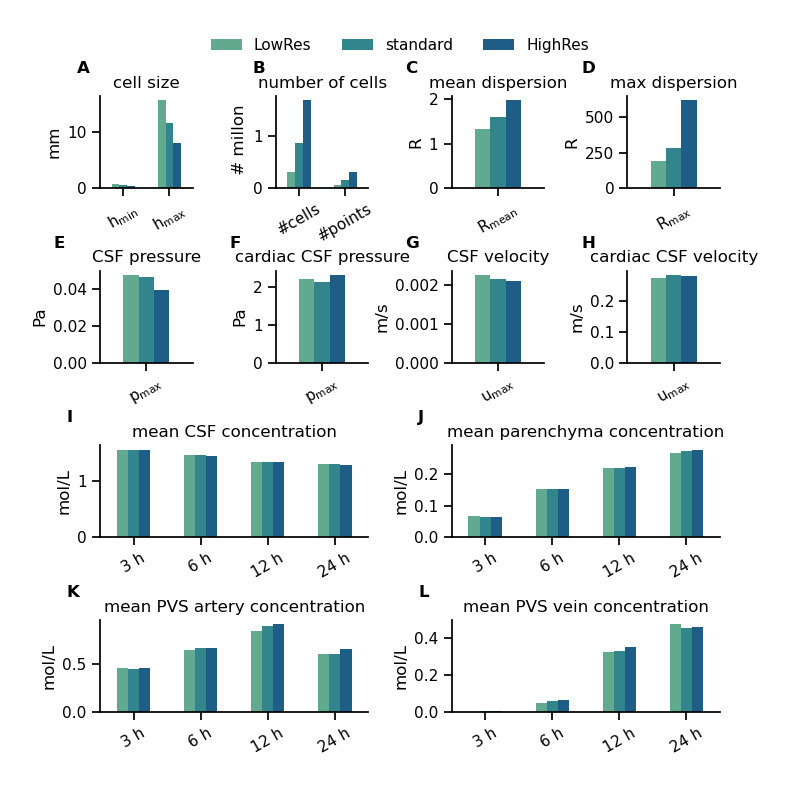
\includegraphics[width=0.9\linewidth]{figures/mesh_refinement.png}
    \caption{Illustration of the three different meshes; from left to right: low resolution, standard resolution, high resolution.}
    \label{fig:mesh_refinement}
\end{figure}

\begin{figure}
    \centering
    \begin{subfigure}[b]{0.45\textwidth}
        \centering
        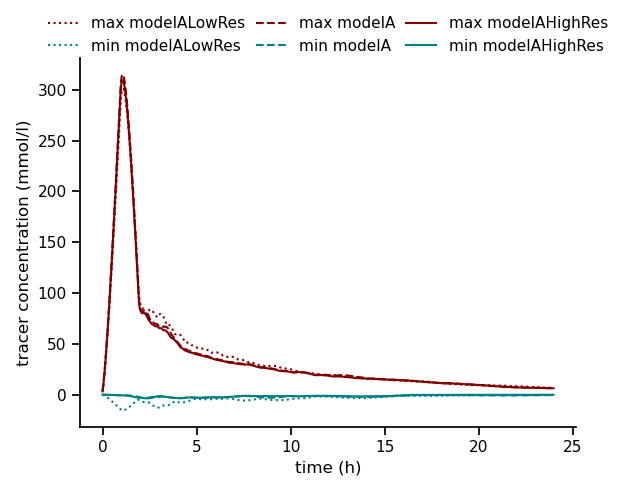
\includegraphics[width = 1 \linewidth]{figures/csf_minmax.png}
        \caption{Minimum and maximum tracer concentration in the CSF under mesh refinement}
    \end{subfigure}
    \begin{subfigure}[b]{0.45\textwidth}
        \centering
     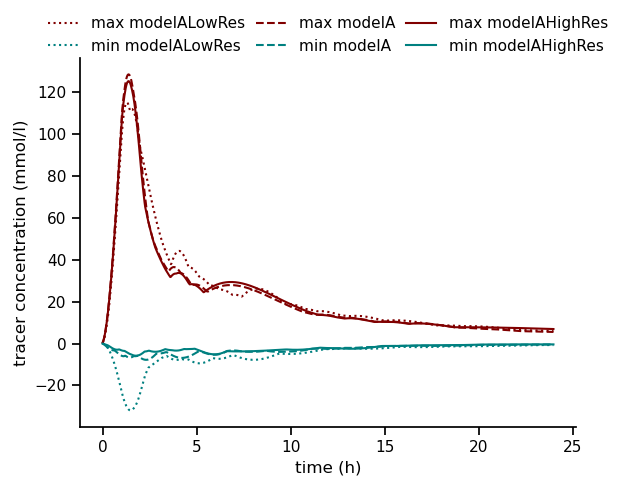
\includegraphics[width= 1 \linewidth]{figures/par_minmax.png}
        \caption{Minimum and maximum tracer concentration in the parenchyma under mesh refinement}
    \end{subfigure}
    \begin{subfigure}[b]{0.45\textwidth}
        \centering
        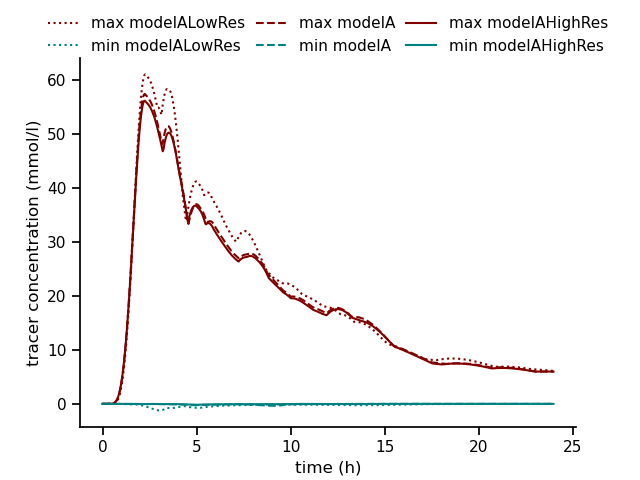
\includegraphics[width = 1 \linewidth]{figures/art_minmax.png}
        \caption{Minimum and maximum tracer concentration in PVSs around arteries under mesh refinement}
    \end{subfigure}
    \begin{subfigure}[b]{0.45\textwidth}
        \centering
     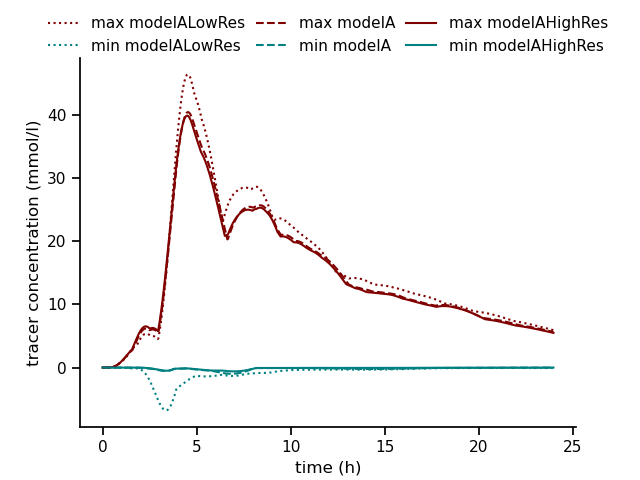
\includegraphics[width= 1 \linewidth]{figures/ven_minmax.png}
         \caption{Minimum and maximum tracer concentration in PVSs around veins under mesh refinement}
    \end{subfigure}
    \caption{Minimum and maximum tracer concentrations over the first 24\,h after injection on the CSF and parenchyma (a), and the arterial and venous PVS (b) computed on the low resolution (LowRes), standard and high resolution (HighRes) meshes with a timestep of 2 min for the baseline model (Model A).}
    \label{fig:mesh_convergence_concentrations}
\end{figure}
\begin{figure}
    \centering
    \begin{subfigure}[b]{0.49\textwidth}
        \centering
        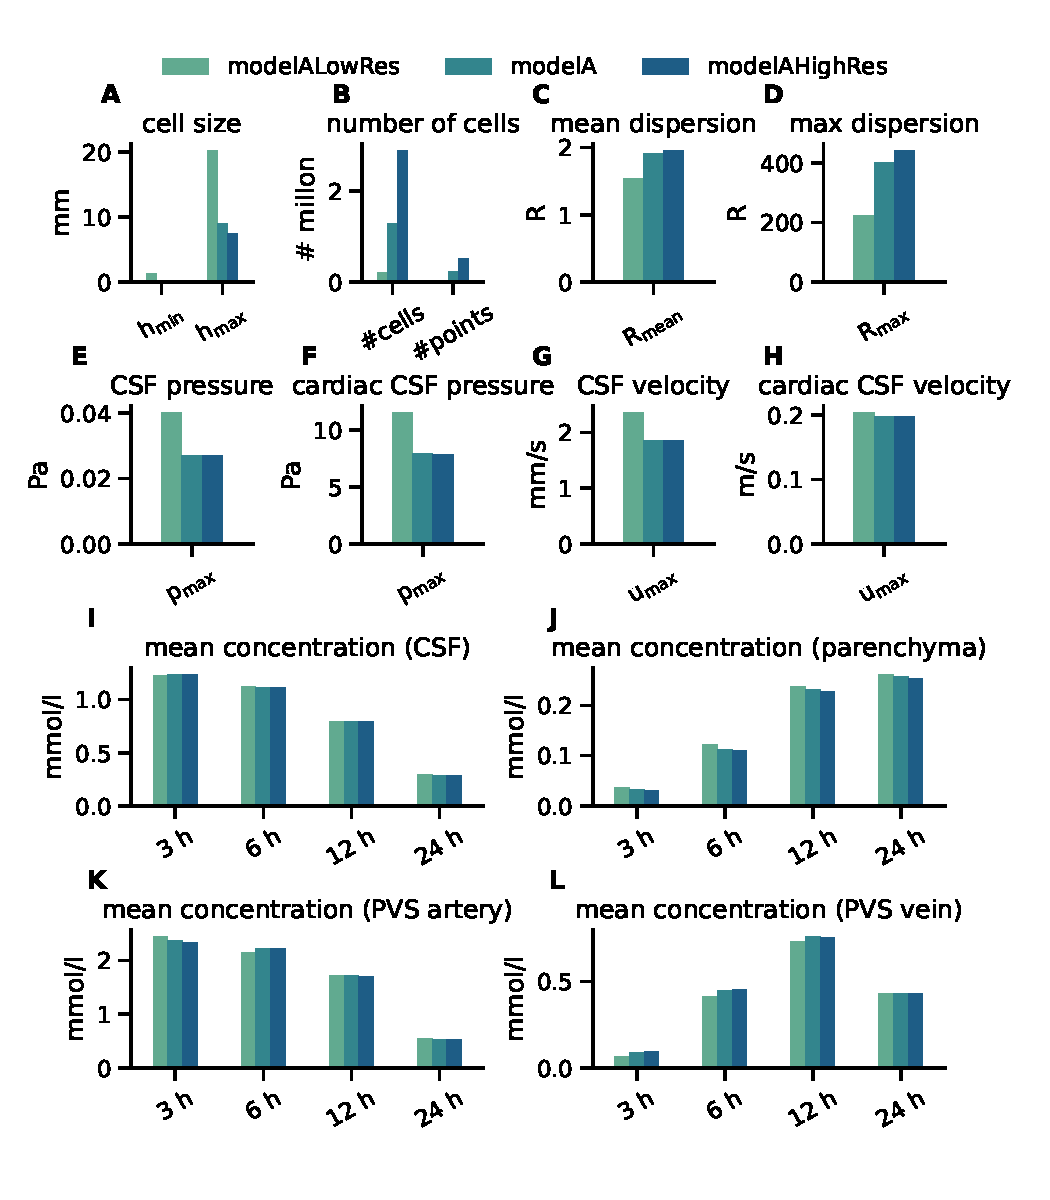
\includegraphics[trim={0.5cm 1cm 0.05cm 0.8cm}, clip, width = 1.05 \linewidth]{figures/modelALowRes_modelA_modelAHighRes.pdf}
        \caption*{Convergence of key quantities of interest with mesh refinement}
        %\label{fig:mesh_convergence}
    \end{subfigure}
    \begin{subfigure}[b]{0.49\textwidth}
        \centering
     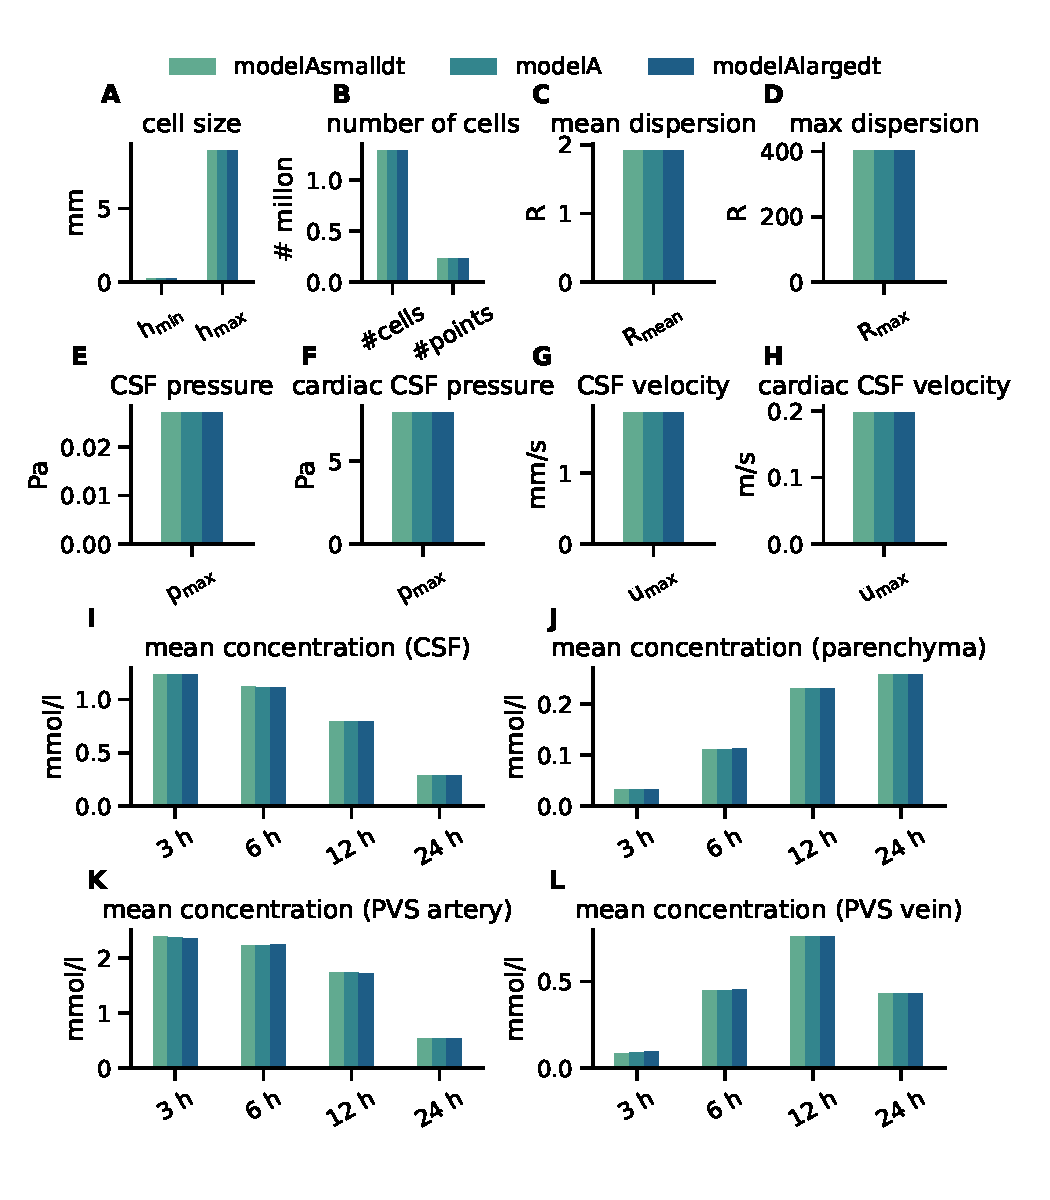
\includegraphics[trim={0.5cm 1cm 0.05cm 0.8cm}, clip,width= 1.05 \linewidth]{figures/modelAsmalldt_modelA_modelAlargedt.pdf}
        \caption*{Convergence of key quantities of interest with time refinement}
        %\label{fig:time_convergence}
    \end{subfigure}
    \caption{For both left and right panels: A: Minimal ($\rm h_{min}$) and maximal ($\rm h_{max}$) mesh cell sizes (computed as cell circumradius $\times 2$); B: number of mesh vertices and tetrahedral cells in each mesh; C: mean cardiac dispersion enhancement factor $R$; D: maximum cardiac dispersion enhancement factor $R$; E: maximum pressure in steady CSF production flow; F: maximum pressure in cardiac-driven CSF flow; G: maximum CSF velocity in steady CSF production flow; H: maximum CSF velocity in cardiac-driven CSF flow; I--L: mean tracer concentration in the CSF, parenchyma, arterial PVS and venous PVS after 3, 6, 12 and 24 hours.}
        \label{fig:mesh_time_convergence}
\end{figure}

\begin{figure}
    \centering
    \begin{subfigure}[b]{0.45\textwidth}
        \centering
        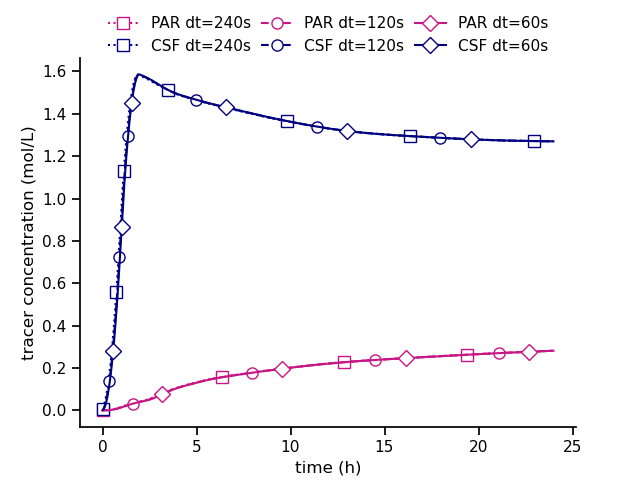
\includegraphics[width = 1 \linewidth]{figures/time_refinement_par_csf_mean.png}
        \caption{Mean tracer concentration in CSF and parenchyma under time step refinement}
    \end{subfigure}
    \begin{subfigure}[b]{0.45\textwidth}
        \centering
     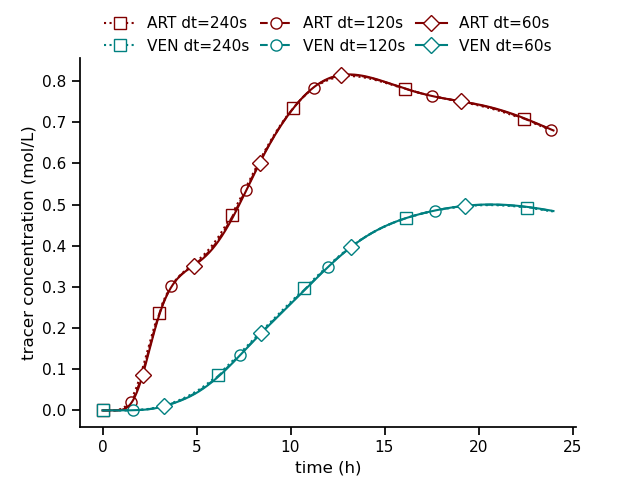
\includegraphics[width= 1\linewidth]{figures/time_refinement_art_ven_mean.png}
         \caption{Mean tracer concentration in PVSs around (veins and) arteries under time step refinement}
    \end{subfigure}
    \caption{Mean tracer concentrations after up to 24\,h in the CSF and parenchyma (a), and the arterial and venous PVS (b) computed on the standard resolution mesh for timesteps of 1, 2, and 4 minutes (dt of 60, 120, or 240 seconds)}
    \label{fig:time_convergence_concentrations}
\end{figure}
\begin{figure}
    \centering
    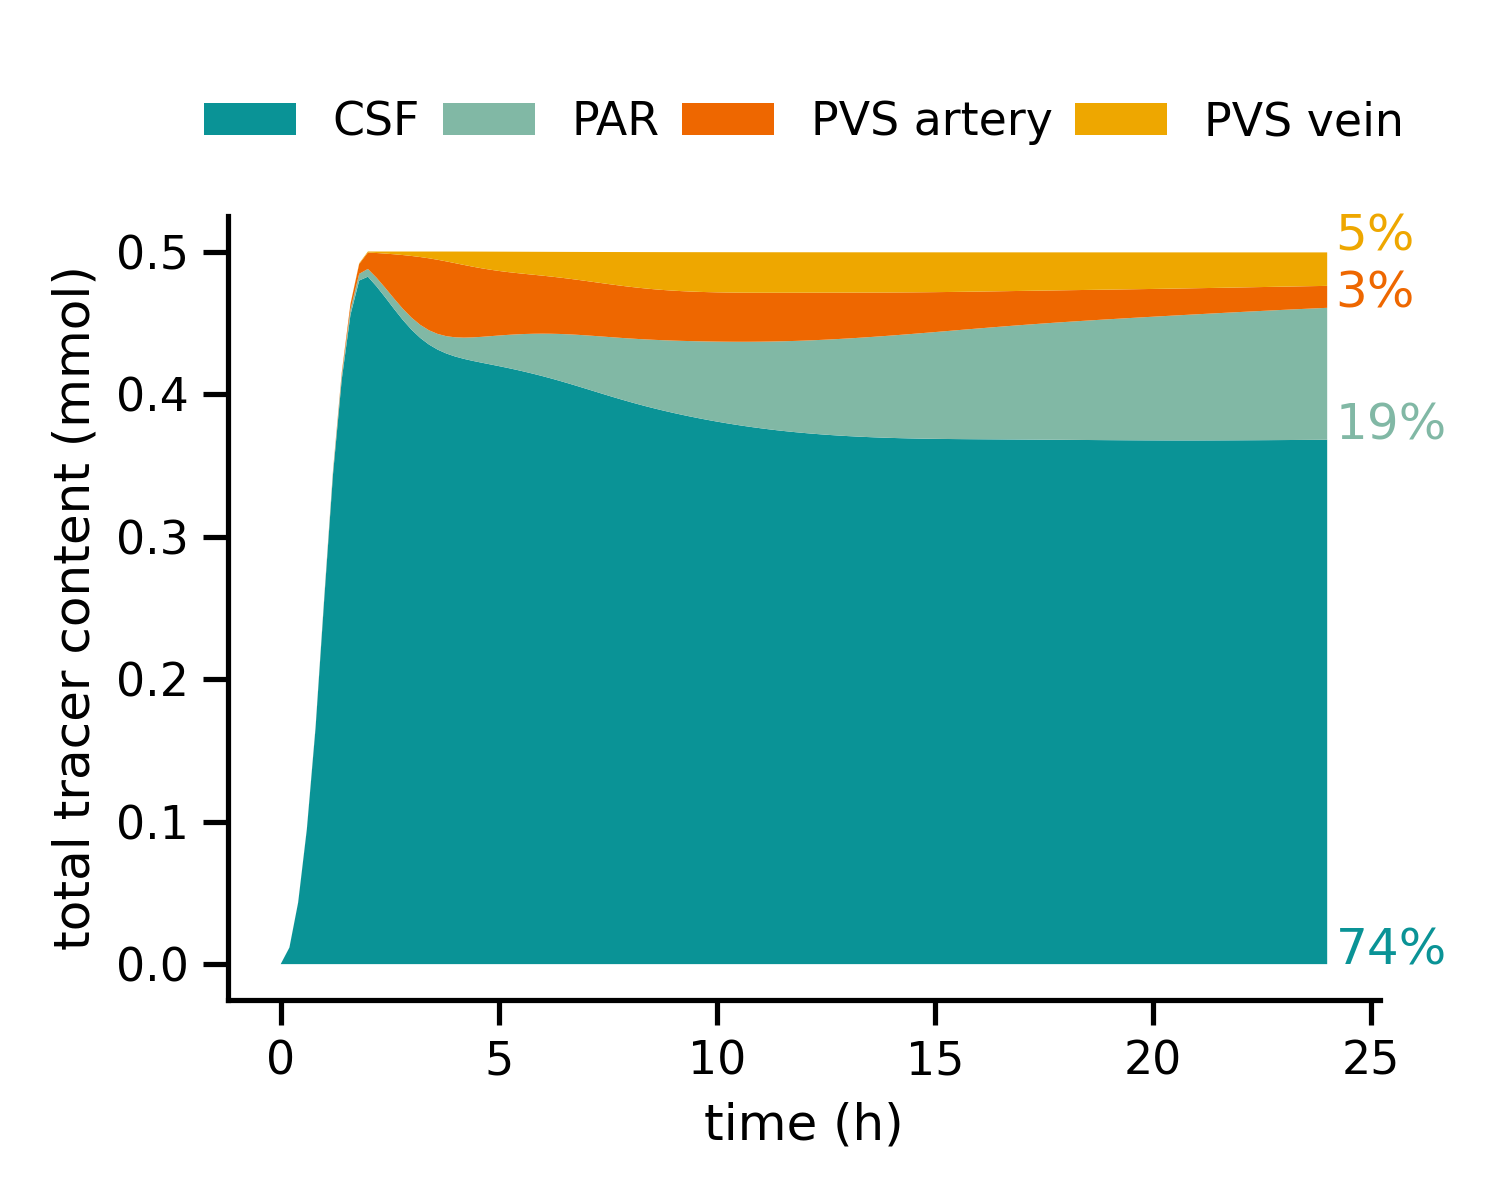
\includegraphics[width=0.5\linewidth]{figures/modelAMassConservation_total_conc.png}
    \caption{Total tracer content in the CSF, parenchyma, and arterial and venous PVS for a variant of the baseline model without tracer outflow. The total amount of tracer is constant after the initial influx phase demonstrating that the numerical scheme conserves mass globally.}
    \label{fig:mass_conservation}
\end{figure}

\section{Supplementary discussion}

\subsection{Extended model validation}
\label{sec:app:model_validation}

In addition to the comparison of our in-silico predictions of tracer
enrichment and clearance against glymphatic MRI, we here compare
auxiliary model quantities against the literature as additional model
validation.

\paragraph{CSF flow and pressures in the SAS and ventricular system}
The dynamics of human CSF flow and pressure are better quantified, by
way of clinical imaging, in-vitro studies, and computational
modelling, in other areas of the ventricular
system~\cite{linninger2007cerebrospinal, sweetman2011cerebrospinal,
  vinje2019respiratory, hornkjol2022csf, causemann2022human,
  karki2025real, liu2025transmantle}. Linninger et
al~\cite{linninger2007cerebrospinal} model CSF flow and pressure
dynamics induced by CSF production and cardiac pulsatility under
normal and hydrocephalic conditions, and report of very good agreement
with Cine (phase-contrast) MRI measurements. Our estimates of the
maximum intracranial pressure difference, 10 Pa from the cardiac
contribution and 26 mPa from CSF production, is in perfect agreement
with their maximum transmantle pressure difference of $\sim$10 Pa, and
also in very good agreement with mean pressure differences of 11.5 Pa
measured clinically between sensors placed subdurally and in the
lateral ventricle \cite{vinje2019respiratory}. Liu et
al~\cite{liu2025transmantle} report of cardiac and respiratory
pressure differences across the aqueduct of 12.1 $\pm$ 5.7 Pa and 9.5
$\pm$ 7.2 Pa, respectively; thus our baseline estimate of the respiratory contribution 1.4 Pa may be an
underestimation. On the other hand, our cardiac- and
respiratory-driven CSF flow estimates peak at 19.8 cm/s and 4.8 cm/s in the caudal direction, respectively, which are higher than phase-contrast MRI measurements of cardiac and respiratory CSF flow
components \cite{takizawa2017characterization, yildiz2017quantifying}. Some variation in CSF flow velocities is expected considering that the values from MRI represent averages
\cite{yildiz2017quantifying} and that the geometry of the CSF spaces
strongly affects peak velocities\cite{vinje2019respiratory,
  causemann2022human}. Hornkjøl et al \cite{hornkjol2022csf} model the
flow dynamics induced by CSF production in the choroid plexus and
report a peak CSF velocity of 8.9 mm/s in the aqueduct, which is 4.8
$\times$ higher than our values of 1.85 mm/s. Given that we use the
same production rate, this deviation again illustrates the impact of
potential differences in the (aqueduct) geometry on local velocities.

% Dispersion predictions
\paragraph{Dispersion in the SAS, ventricular system and PVS}
This pulsatile flow of CSF in the SAS, ventricular system and PVSs
leads to an increase in effective solute
diffusivity~\cite{stockman2007effect, hettiarachchi2011effect,
  asgari2016glymphatic, sharp2019dispersion, ray2021quantitative} via
a process known as Taylor dispersion \cite{taylor1953dispersion,
  watson1983diffusion}. Previous estimates of the magnitude of this
effect in the CSF spaces vary significantly: from an enhancement
factor of 0.05--1 in periarterial spaces surrounding penetrating
arteries~\cite{asgari2016glymphatic, troyetsky2021dispersion}, to
5--100 in the spinal subarachnoid space~\cite{stockman2007effect,
  hettiarachchi2011effect, sharp2019dispersion}, and up to more than
$10\,000$ in surface periarterial spaces~\cite{ray2021quantitative,
  sharp2019dispersion}. The large variability can (at least partly) be
attributed to methodological differences; e.g. different assumptions
on the medium, domain width, pressure differences and/or fluid
velocities, the diversity of CSF flow characteristics, as well as a
high likelihood of spatial variations. Hornkjøl et
al~\cite{hornkjol2022csf} consider model variations with constant
dispersion factors from 1 up to 1000, and indicate that a value of 10
gives the better agreement with the clinically observed
enrichment. Our spatially-varying estimates of the dispersion
enhancement factors $R_c, R_r$ (with $D = (1 + R_c + R_r) D^{\rm
  Gad}$) range from 0 to 200 for the cardiac contribution $R_c$ and 0
to 320 for the respiratory contribution $R_r$; and is thus compatible
within the previously reported spectrum.

% Effect of PVS size and shapes
\paragraph{Shapes, sizes and structures of the PVS}
The shapes, sizes and structures of the PVSs likely vary between
species (e.g.~mice vs.~humans), between spatial compartments
(e.g.~surface vs.~parenchymal), between vessel types (arteries
vs.~arterioles vs.~veins), and in
pathologies~\cite{ichimura1991distribution, foley2012realtime,
  schain2017cortical, mestre2018flow, bedussi2018paravascular,
  mestre2022periarteriolar, smets2024perivascular, raicevic2023sizes,
  vinje2021brain, eide2024functional}. In terms of shape, the PVSs are
commonly represented as annular (elliptic) cylinders, though it is
well recognized that this represents an
idealization~\cite{mestre2018flow, tithof2019hydraulic,
  vinje2021brain, raicevic2023sizes, boster2024hydraulic,
  smets2024perivascular}. In terms of sizes, Raicevic et
al~\cite{raicevic2023sizes} note that the variation in PVS area is
larger between PVS segments than along a single PVS segment and that
the PVS area increases with lumen area. In mice, reports of the ratio
between PVS and lumen area range from
$\approx$0.35--0.43~\cite{smets2024perivascular} up to
$\approx$1.12--1.4~\cite{raicevic2023sizes, mestre2018flow}. In
humans, the PVS may be as wide as the associated surface artery and up
to 4$\times$ wider in iNPH subjects~\cite{eide2024functional}, which
would correspond to substantially larger PVS area ratios (3 or
higher). To reflect the human scale, we here represent each PVS
segment as an annular cylinder with inner radius $R_1$ and outer
radius $R_2$ of width and area proportional to that of the
corresponding blood vessel ($R_2 = 2 R_1$ at baseline, $R_2 = 3 R_1$
for enlarged PVS). The hydraulic resistance of annular cross-sections
is $1-6 \times$~\cite{tithof2019hydraulic} larger than more elongated
cross-sections and thus our estimates of the pressure-induced PVS
velocities are conservative.

%\paragraph{Predictions on overall tracer spreading patterns}

%We compare our in-silico predictions with clinical data from human subjects, in particular the studies by Ringstad et al~\cite{ringstad2018brain}, Watts et al~\cite{watts2019measuring} and Eide and Ringstad~\cite{eide2024functional}. Finding an overall good agreement, we provide a detailed overview on key quantities of interest in %FTA in MCA2 & N/A & N/A & 53.1 ± 50.5 min & 2:12 / 1:48 hours +$t_{st}$ \\
%FTA in ACA2 & N/A & N/A & 48.3 ± 46.1 min & 3:00 hours +$t_{st}$ \\
%\bottomrule
%\end{tabular}
%\caption{Comparison of clinical studies and model predictions on tracer spreading patterns %and arrival times.}
%\label{tab:spreading_comparison}
%\end{table}
